%!TEX root = ../main.tex


Στο κεφάλαιο ~\ref{ch:chap1} έγινε μια σύντομη εισαγωγή στις βιολογικές έννοιες των πρωτεϊνών και των πρωτεϊνικών αλληλεπιδράσεων, που αποτελούν το αντικείμενο της συγκεκριμένης εργασίας. Στη συνέχεια, στο κεφάλαιο ~\ref{ch:chap2} παρουσιάστηκαν οι έννοιες της μηχανικής μάθησης και των νευρωνικών δικτύων, τα οποία αποτέλεσαν τα εργαλεία που χρησιμοποιήθηκαν για την εκπόνηση της παρούσας εργασίας. Στο συγκεκριμένο κεφάλαιο παρουσιάζεται η προσέγγιση που επιλέχθηκε για την επίλυση του προβλήματος του εντοπισμού πρωτεϊνικών αλληλεπιδράσεων με τη χρήση μοντέλων μηχανικής μάθησης και συγκεκριμένα νευρωνικών δικτύων. Αρχικά, γίνεται μια ανάλυση του συγκεκριμένου προβλήματος το οποίο πρέπει να επιλυθεί και αναφέρεται αναλυτικά η διαδικασία εξαγωγής βιολογικών δεδομένων για τις ανάγκες του μοντέλου μας. Γίνεται λεπτομερής περιγραφή των διαδικασιών προεπεξεργασίας προκειμένου τα δεδομένα να μετασχηματιστούν στην κατάλληλη μορφή για την εκπαίδευση των διαφόρων μοντέλων. Ταυτόχρονα, παρουσιάζονται τα εργαλεία που χρησιμοποιήθηκαν για την ανάπτυξη των μοντέλων. Παράλληλα, παρουσιάζεται υλοποίηση μεθόδου παραγοντοποίησης μητρώων ( \textit{matrix factorization} ) καθώς και τεχνική αποδόμησης τανυστή (\textit{tensor decomposition} προκειμένου να συμπληρωθούν τυχών μη έγκυρες τιμές. Τέλος, αναλύονται οι αρχιτεκτονικές νευρωνικών δικτύων που υλοποιήθηκαν, οι λόγοι για τους οποίους επιλέχθηκαν καθώς και περαιτέρω παρατηρήσεις πάνω στο συγκεκριμένο πρόβλημα.

\newpage
\section{Ορισμός προβλήματος}

Οπως αναφέρθηκε προηγουμένως, οι αλληλεπιδράσεις μεταξύ πρωτεϊνών παίζουν καθοριστικό ρόλο στις λειτουργίες των πρωτεϊνών, επιτρέποντας τους να εκτελέσουν τις βασικές βιολογικές διαδικασίες της ζωής των οργανισμών. Οι πρωτεΐνες αλληλεπιδρούν μεταξύ τους μέσω των \textit{inter\-faces}, που αποτελούν περιοχές της επιφάνειάς τους με συγκεκριμένες γεωμετρικές και φυσικοχημικές ιδιότητες. Επομένως, το πρώτο βήμα για τον εντοπισμό πρωτεϊνικών αλληλεπιδράσεων είναι η εύρεση πληροφοριών σχετικά με πρωτεϊνικά interfaces.

\medskip
\begin{figure}[h]
  \centering
  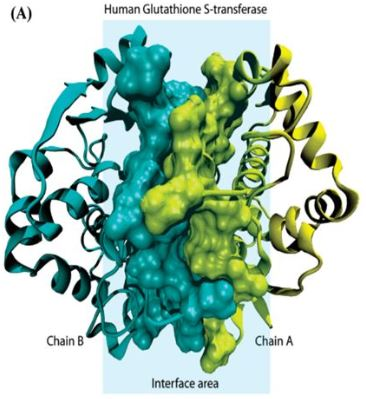
\includegraphics[scale=1]{images/protein interface.JPG}
  \caption{Παράδειγμα επιφάνειας αλληλεπίδρασης σε PPI}
  \label{fig:protein interface}
\end{figure}

\medskip
Η βασικότερη πηγή δεδομένων σχετικά με πρωτεϊνικά interfaces προέρχεται από τις πρωτεϊνικές δομές που είναι αποθηκευμένες στην \textit{Protein Data Bank} και συγκεκριμένα εξάγονται μέσω X-ray crystallography. Ωστόσο, ο προσδιορισμός interfaces μέσω της παραπάνω βάσης δεδομένων αποτελεί μια χρονοβόρα και κοστοβόρα διαδικασία, ενώ παράλληλα μόνο το 50\% των δομών που περιέχονται στην PDB είναι αλληλεπιδράσεις πρωτεϊνών, με το άλλο 50\% να είναι μονομερή, νουκλεοτιδικές αλυσίδες κ.α. Ακόμη, μονάχα ένα μικρό κομμάτι από τις πρωτεϊνικές αλληλεπιδράσεις που περιέχονται στην PDB αποτελούν πραγματικές βιολογικές δομές, επομένως η επιβεβαίωση των πρωτεϊνικών αλληλεπιδράσεων με έναν τρόπο υψηλής ακρίβειας αποτελεί δύσκολο πρόβλημα. Παράλληλα, η φύση της X-ray κρυσταλλογραφίας οδηγεί στην αποτύπωση κρυσταλλικών δομών που περιέχουν βιολογικά ασήμαντες κρυσταλλικές επαφές ή δεν περιέχουν σχετικές επαφές που υπάρχουν, με αποτέλεσμα την ανάγκη επαναπροσδιορισμού και διαχωρισμού των πραγματικών βιολογικών επαφών από τις κρυσταλλικές επαφές μεταξύ των πρωτεϊνών.

\medskip
Για τους παραπάνω (και όχι μόνο) λόγους, δημιουργήθηκε η ανάγκη πρόβλεψης πρωτεϊνικών αλληλεπιδράσεων \textit{in silico} προκειμένου να κατανοήσουμε περαιτέρω τις βιολογικές διαδικασίες αλλά και να διευρύνουμε την γνώση πάνω στον τομέα της κατασκευής φαρμάκων \cite{Fletcher2006}. 

\medskip
Υπάρχει ήδη ένας μεγάλος αριθμός μεθόδων για τον προσδιορισμό PPIs, με τις περισσότερες να εφαρμόζουν αλγορίθμους μηχανικής μάθησης πάνω σε σετ χαρακτηριστικών που εξάγονται από την ακολουθιακή ομολογία ή/και τη δομή των πρωτεϊνών με γνωστά interfaces (δηλαδή είναι χαρακτηριστικά sequence-based ή/και structure-based, που αναλύθηκαν στο κεφάλαιο ~\ref{ch:chap1} ). Οι μέθοδοι διαφέρουν στα δεδομένα που χρησιμοποιούν για την εκπαίδευση και αξιολόγηση των αλγορίθμων, στην φύση των interfaces (αν δηλαδή είναι transient η/και obligate), στην φύση των προβλέψεων, στην επιλογή των residues για αξιολόγηση και άλλα. Στη συγκεκριμένη διπλωματική, παρουσιάζεται μια τεχνική μηχανικής μάθησης που εκπαιδεύεται σε sequence-based και structure-based χαρακτηριστικά και προβλέπει αλληλεπιδράσεις πρωτεϊνών τόσο σε επίπεδο patch οσο και σε επίπεδο residue. 

\section{Δεδομένα} \label{data}
\subsection{Ανάκτηση δεδομένων πρωτεϊνικών αλληλεπιδράσεων}

Η εξαγωγή του σετ δεδομένων βασίζεται σε επιστημονική εργασία που δημοσιεύτηκε το 2017 με τίτλο \textit{IntPred: a structure-based predictor of protein-protein interaction sites} \cite{Northey2017} και ακολουθήθηκε η ίδια διαδικασία προκειμένου τα αποτελέσματα να είναι συγκρίσιμα.

\medskip
Όπως αναφέρθηκε προηγουμένως, η φύση της X-ray κρυσταλλογραφίας οδηγεί στην αποτύπωση επαφών που δεν έχουν βιολογική σημασία. Για τον λόγο αυτό, χρησιμοποιείται το εργαλείο \textit{PISA} (\textit{\textbf{P}rotein, \textbf{I}nterfaces, \textbf{S}tructures and \textbf{A}ssemblies}), που εξάγει δεδομένα από την PDB και χρησιμοποιώντας μεθόδους χημικής θερμοδυναμικής διαχωρίζει τις συγκεντρώσεις μακρομορίων από τις κρυσταλλικές επαφές \cite{Krissinel2007}. Μέσω του εργαλείου PISA, ανακτήθηκαν \textbf{58,397} βιολογικές μονάδες.

\medskip
\begin{figure}[h]
  \centering
  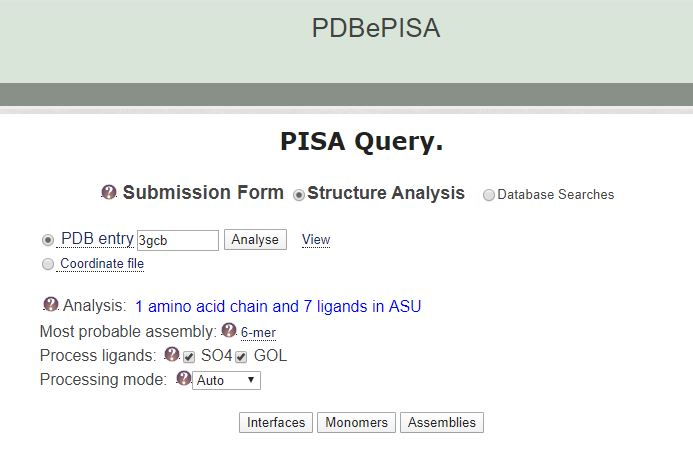
\includegraphics[scale=0.7]{images/PISA.JPG}
  \caption{Εργαλείο PISA}
  \label{fig:PISA}
\end{figure}

\medskip
Στη συνέχεια πραγματοποιήθηκε ένας "καθαρισμός" των αποτελεσμάτων που ανακτήθηκαν. Αρχικά, διαγράφηκαν αποτελέσματα που περιείχαν πρωτεϊνικά περιβλήματα ιών (\textit{viral capsids}) καθώς και αποτελέσματα που προέκυψαν μέσω NMR spectroscopy (η διαδικασία περιγράφηκε στο κεφάλαιο ~\ref{ch:chap1} ). Ακόμη, για λόγους ποιότητας των αποτελεσμάτων διαγράφηκαν αποτελέσματα με ανάλυση χειρότερη των 3\AA   ή R-factor μεγαλύτερο του 30\% . R-factor είναι μια μετρική ομοιότητας μεταξύ ενός κρυσταλλογραφικού μοντέλου και των πειραματικών X-ray αποτελεσμάτων διάθλασης, όπου ουσιαστικά υποδεικνύει την ποιότητα του μοντέλου κρυσταλλογραφίας. Για ανάλυση μεγαλύτερη από 2\AA, το R-factor δεν πρέπει να υπερβαίνει σημαντικά το 0.25. Τέλος, αφαιρέθηκαν τυχών πεπτιδικές αλυσίδες που προέκυψαν μέσω της ανάκτησης των αποτελεσμάτων (δηλαδή δομές με λιγότερα από 30 αμινοξέα). Με αυτό τον τρόπο, από τα αρχικά \textbf{58,397} αποτελέσματα προέκυψαν \textbf{25,876} δομές κατασκευασμένες από \textbf{87,738} αλυσίδες.

\medskip
Επιπλέον, για την αποφυγή πανομοιότυπων ή παρόμοιων αποτελεσμάτων σε διαφορετικά entries, χρησιμοποιήθηκε το εργαλείο \textit{PISCES}. Το \textit{PISCES} (A Protein Sequence Culling Server) είναι ένα εργαλείο που δημιουργεί υποσύνολα υψηλής ποιότητας από μεγάλα σετ πρωτεϊνών, με βάση μια πληθώρα παραγόντων όπως η δομική ποιότητα, η μέγιστη κοινή ακολουθία ταυτοτήτων κ.α. Μέσω του εργαλείου PISCES, ομαδοποιήθηκαν οι αλυσίδες κατά 25\% ακολουθιακή ομοιότητα (sequence simularity) και στη συνέχεια από κάθε ομάδα επιλέχθηκε ο καλύτερος "αντιπρόσωπος" με βάση την ποιότητα ανάλυσης ή (σε περίπτωση ισοβαθμίας) του καλύτερου R-factor. Έτσι, καταλήξαμε σε \textbf{4,345} αλυσίδες.


\begin{figure}[h]
  \centering
  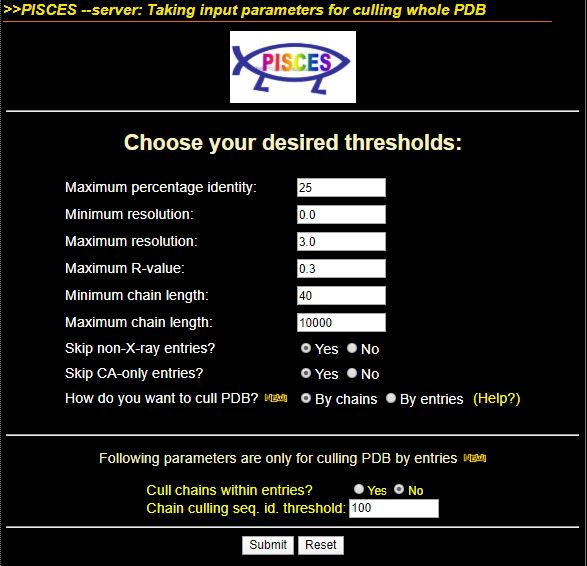
\includegraphics[scale=0.8]{images/PISCES.JPG}
  \caption{Εργαλείο PISCES}
  \label{fig:PISCES}
\end{figure}

\medskip
Η παραπάνω διαδικασία που περιγράφηκε αφορά την εξαγωγή των δεδομένων εκπαίδευσης εκτελέσθηκε ξεχωριστά και για τη δημιουργία του σετ αξιολόγησης, το οποίο περιείχε \textbf{4204} αλυσίδες.

\subsection{Δημιουργία κομματιών επιφάνειας}

Προκειμένου να υπολογιστούν οι ιδιότητες της πρωτεϊνικής επιφάνειας, η επιφάνεια πρέπει να διαιρεθεί σε μικρότερα μέρη (fragments). Για τον σκοπό αυτό χρησιμοποιήθηκε το πρόγραμμα \textit{pdbmakepatch}, που ανήκει στο σύνολο προγραμμάτων υπολογιστικής βιολογίας \textit{BiopTools} και αναπτύχθηκε το 2015 από το πανεπιστήμιο UCL \cite{Porter2015}, το οποίο εξάγει κομμάτια επιφάνειας από δοθείσες πρωτεΐνες.

\medskip
Ειδικότερα, προτού αναλυθεί η λειτουργία του προγράμματος, πρέπει να γίνει μια εισαγωγή στους ακόλουθους όρους:

\medskip
\begin{itemize}
    \item \textbf{Patch centre atom} : Είναι το άτομο που δίνεται ως είσοδος στο πρόγραμμα και με βάση το οποίο υπολογίζονται τα κομμάτια (patches) της επιφάνειας. \\
    \item \textbf{Patch radius} : Είναι η ελάχιστη απόσταση με βάση την οποία επιλέγονται τα υποψήφια residues για το τελικό κομμάτι. \\
    \item \textbf{Contact radius} : Ορίζεται για ένα ζεύγος ατόμων ώς το άθροισμα των ακτίνων Van der Waals τους, συν έναν παράγοντα σφάλματος (στο συγκεκριμένο πρόβλημα ορίζεται στα 2 \AA ). Δύο άτομα θεωρούμε ότι βρίσκονται σε \textit{επαφή} αν η απόσταση των κέντρων τους είναι μικρότερη από το contact radius. \\
    \item \textbf{Residue geometry vector} : Πρόκειται για έναν πίνακα που ορίζεται για δοσμένα residue ξεκινώντας από το κέντρο του ατόμου ( C\textsubscript{a} ) και τερματίζοντας στο γεωμετρικό κέντρο των 10 γειτονικά πλησιέστερων residues. Το γεωμετρικό κέντρο ορίζεται ως ο μέσος όρος των συντεταγμένων των κέντρων τους. \\
    \item \textbf{Residue solvent vector} : Πίνακας με παρόμοια αρχή όπως ο residue geometry vector, ωστόσο κινείται στην αντίθετη κατεύθυνση. \\
    \item \textbf{Solvent angle} : Ορίζεται για ένα ζεύγος residues ως η γωνία μεταξύ των residue solvent vectors τους. \\
\end{itemize}

\medskip
Για ένα δοσμένο αρχείο pdb και ένα patch centre atom, το πρόγραμμα \textit{pdbmakepatch} δημιουργεί ένα κομμάτι ακολουθώντας την εξής επαναληπτική διαδικασία:

\medskip
\begin{enumerate}
    \item Ορίζεται \textit{P} ενα αρχικά άδειο σύνολο ατόμων του κομματιού και προσθέτουμε το patch centre atom στο \textit{P}. \\
    \item Βρίσκουμε όλα τα residues με τουλάχιστον ένα κέντρο ατόμου μέσα στην ακτίνα (patch radius) του κεντρικού ατόμου (patch centre atom). Τα συγκεκριμένα residues αποτελούν το σύνολο \textit{C} των υποψήφιων για εισαγωγή στο κομμάτι. \\
    \item Για κάθε μέλος του συνόλου \textit{P}, ελέγχουμε αν υπάρχει επαφή με κάποιο από τα μέλη του συνόλου \textit{C}. Αν κάποιο μέλος του συνόλου \textit{C} βρίσκεται σε επαφή με μέλος του \textit{P} και το solvent angle που σχηματίζουν είναι μικρότερο από 120\degree , τότε το μεταφέρουμε στο \textit{P}. \\
    \item Επαναλαμβάνουμε το βήμα 3 μέχρις ότου να μην υπάρχει μεταφορά μελών από το σύνολο \textit{C} στο σύνολο \textit{P}. \\
    \item Κάθε residue με άτομο στο σύνολο \textit{C} ορίζεται ως \textit{patch residue}. \\
\end{enumerate}


\bigskip
Η χρήση του solvent angle γίνεται για να μην συμπεριληφθούν residues από αντίθετες πλευρές στο ίδιο κομμάτι, με αποτέλεσμα τη δημιουργία διακεκομμένων κομματιών, οπως φαίνεται στην παρακάτω εικόνα. Το άτομο υποψήφιος (κόκκινο) βρίσκεται εντός της απόστασης επαφής (contact radius) από ένα άτομο που ανήκει στο κομμάτι (μωβ). Οι residue geometry vectors (άσπρο) χρησιμοποιούνται για να υπολογιστούν οι solvent angle vectors (μαύρο), με βάση τους οποίους υπολογίζεται το solvent angle. Στη συγκεκριμένη περίπτωση, καθώς η γωνία ξεπερνά τις 120\degree , το άτομο υποψήφιος δεν συμπεριλαμβάνεται στο κομμάτι. 

\medskip
\begin{figure}[h]
  \centering
  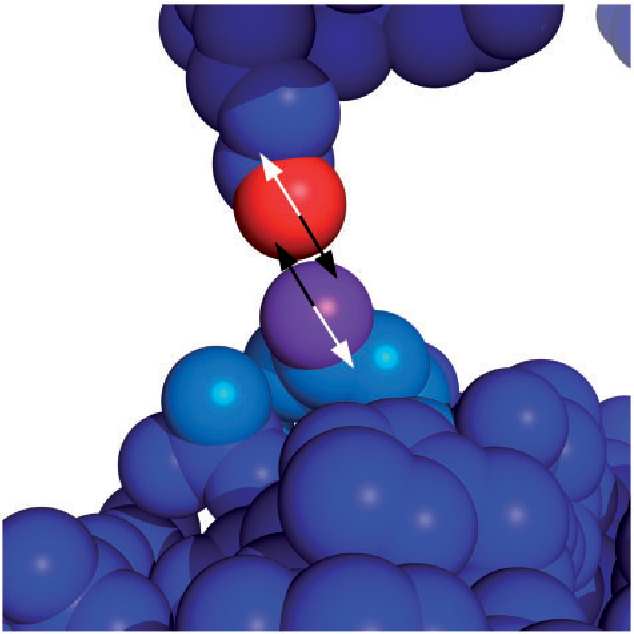
\includegraphics[scale=0.5]{images/solvang.png}
  \caption{Παράδειγμα χρήσης solvent angle}
  \label{fig:solvang}
\end{figure}

\medskip
Για όλες τις δομές που προέκυψαν κατά την δημιουργία των δεδομένων εκπαίδευσης, δημιουργούνται σετ επικαλυπτόμενων κομματιών (\textit{overlapping patches}) για να απεικονισθεί η επιφάνειά τους. Για να δημιουργηθούν τα παραπάνω σετ, επιλέχθηκαν residues με \textit{relative solvent accessibility} (\textit{RSA}) > 25\%. Η συγκεκριμένη μετρική, που ονομάζεται και σχετικά προσβάσιμη επιφάνεια (relative solvent accessible area - RASA ), αποτελεί μια μετρική έκθεσης ενός residue και υπολογίζεται με τον ακόλουθο τύπο:

\begin{equation}
    RASA = \frac{ASA}{max(ASA)} 
\end{equation}
where:


{
\centering
\begin{conditions}
   ASA & προσβάσιμη επιφάνεια από διαλυτικό μέσο . \\
   max(ASA) & μέγιστη δυνατή προσβάσιμη επιφάνεια για το residue. \\
\end{conditions}}

Τα παραπάνω επιλεγμένα residues αποτελούν το σύνολο των κέντρων κομματιού. Για κάθε residue που ανήκει σε αυτό το σύνολο, το άτομο με την υψηλότερη ASA βρίσκεται και επιλέγεται ως patch centre atom για είσοδο στο πρόγραμμα \textit{pdbmakepatch}.

\subsection{Ανάθεση κατηγορίας}

Για την ανάθεση της κατηγορίας του κάθε κομματιού (class label), υπολογίζεται το ποσοστό της RASA (Relative Solvent Accessible Area) που οφείλεται σε residues τα οποία έχουν χαρακτηριστεί ως residues επιφάνειας. Ένα residue χαρακτηρίζεται ως residue επιφάνειας εαν ικανοποιεί την παρακάτω σχέση:

\begin{equation}
    RASA^n_i - RASA^c_i \geq 10\% 
\end{equation}
where:


{
\centering
\begin{conditions}
   RASA^n_i & non complex RASA τιμή του residue i. \\
   RASA^c_i &  complex RASA τιμή του residue i. \\
\end{conditions}
}

\medskip
Το ποσοστό της RASA που οφείλεται σε residues επιφάνειας, γνωστό και ως interface fraction \textit{$fASA_p$}, για ένα κομμάτι επιφάνειας \textit{p} που περιέχει ένα σύνολο από residues \textit{$r_p$} και ένα υποσύνολο από residues επιφάνειας \textit{$r_intf$} υπολογίζεται από τον ακόλουθο τύπο:

{\Large
\begin{equation}
    fASA_p = \frac{\sum_{j \in r_intf} RASA^n_j}{\sum_{i \in r_p} RASA^n_i} 
\end{equation}}

\medskip
Τελικά,η κατηγορία που δίνεται σε ένα κομμάτι βασίζεται στον παρακάτω κανόνα:

\begin{equation}
    C_p =
    \begin{cases}
    I & \quad if\  fASA_p \geq 0.5 \\ 
    S & \quad if\  fASA_p = 0 \\
    U & \quad otherwise \\
    \end{cases}
\end{equation}
where:


{
\centering
\begin{conditions}
   I &  Interaction \\
   S & Surface \\
   U &  Unlabelled \\
\end{conditions}
}

\medskip
Ο χαρακτηρισμός ενός κομματιού ως \textit{unlabelled}, δηλαδή δίχως κατηγορία, γίνεται σε περιπτώσεις κομματιών που βρίσκονται στο άκρο της αλληλεπίδρασης ( γίνεται περαιτέρω επεξήγηση σε φωτογραφία στη συνέχεια ). Τα κομμάτια που χαρακτηρίζονται έτσι παραλείπονται από την εκπαίδευση του μοντέλου, προκειμένου να διατηρηθεί η δυαδική φύση του προβλήματος κατηγοριοποίησης, ωστόσο περιλαμβάνονται στα δεδομένα αξιολόγησης όταν οι προβλέψεις κομματιού μεταφέρονται σε επίπεδο residues.

Η παρακάτω φωτογραφία περιέχει μια τοποθεσία αλληλεπίδρασης (το περίγραμμα της οποίας τονίζεται με κίτρινο χρώμα). Το κομμάτι με το κυανό χρώμα χαρακτηρίζεται ως κομμάτι αλληλεπίδρασης (interface patch) ενώ το κομμάτι με το κόκκινο χρώμα ως unlabelled καθώς το ποσοστό των residues του κομματιού που εντάσσονται στην αλληλεπίδραση δεν είναι επαρκώς υψηλό. 
\medskip
\begin{figure}[h]
  \centering
  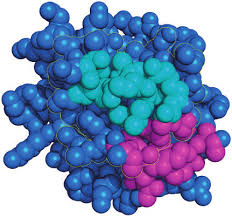
\includegraphics[scale=1.3]{images/unlabelled.jpg}
  \caption{Παράδειγμα unlabelled κομματιού}
  \label{fig:unlabelled}
\end{figure}

\newpage
\subsection{Χαρακτηριστικά δεδομένων}

\medskip
Τα μοντέλα μηχανικής μάθησης που αναπτύχθηκαν για τον εντοπισμό των αλληλεπιδράσεων χρησιμοποίησαν 8 χαρακτηριστικά (\textit{features}) για την εκπαίδευση και την αξιολόγηση τους, τα οποία μπορούν να χωρισθούν σε ακολουθιακά (\textit{sequential}) και δομικά (\textit{structural}) χαρακτηριστικά

\subsubsection{Ακολουθιακά χαρακτηριστικά}

Τα παρακάτω χαρακτηριστικά λαμβάνουν υπόψιν τους μονάχα ακολουθιακές ιδιότητες. Με τον όρο \textit{ακολουθιακό χαρακτηριστικό (sequential feature)} εννοούμε μια ομάδα αμινοξέων μέσα σε μια πρωτεΐνη που παρέχει ορισμένες ιδιότητες. Ορισμένα παραδείγματα ακολουθιακών χαρακτηριστικών είναι τα binding sites καθώς και τα post-translational modification (PTM) sites. Καθώς τα ακολουθιακά χαρακτηριστικά υπολογίζονται σε επίπεδο residues, η τιμή των χαρακτηριστικών για κάθε κομμάτι αποτελεί απλώς τον μέσο όρο των τιμών των residues τους.

\medskip
\begin{itemize}
    \item \textbf{Hydrophobicity}: Η υδροφοβικότητα αποτελεί τη φυσική ιδιότητα ενός μορίου να απωθείται φαινομενικά από μια μάζα νερού. Σε έρευνες που έχουν διεξαχθεί τα τελευταία χρόνια παρατηρείται ότι οι περιοχές αλληλεπίδρασης σε μια πρωτεΐνη είναι πιο υδροφοβικές από την υπόλοιπη πρωτεϊνική επιφάνεια \cite{Jones1997} \cite{Magliery2005}. Για το συγκεκριμένο πρόβλημα, η υδροφοβικότητα ενός residue αντιπροσωπεύεται από την τιμή της στην κλίμακα που ορίστηκε από τους Kyte και Doolittle, η οποία υποδεικνύει υδροφοβικότητα σε αμινοξέα \cite{Kyte1982} και συμφωνα με την οποία περιοχές με θετικές τιμές ορίζονται ως υδροφοβικές. \\
    
    \item \textbf{Propensity}: Ένας άλλος τρόπος διαχωρισμού των συνθέσεων αμινοξέων μεταξύ περιοχών αλληλεπίδρασης και περιοχών επιφάνειας είναι μέσω της ροπής/τάσης των residues (\textit{propensity}). Στο συγκεκριμένο πρόβλημα χρησιμοποιείται η τάση των residues ως προς την ολική προσβάσιμη επιφάνεια (ASA), καθώς αποτελεί ένα απο τα πιο διαδεδομένα χαρακτηριστικά για την μελέτη της λειτουργίας των αλληλεπιδράσεων \cite{Zhou2001}.  Η ροπή ενός residue \textit{i} τύπου \textit{X} υπολογίζεται ως:
    
    {\Large
    \begin{equation}
        Pr(i,X) = (\ln \frac{F_{intf}(X)}{F_{surf}(X)}) \times (\frac{ASA(i)}{\overline{ASA_{surf}} (X)})
    \end{equation}}
    where:
    
    
    {
    \centering
    \begin{conditions}
    F_{intf}(X) & ποσοστό αλληλεπίδρασης του residue τύπου X. \\
    F_{surf}(X) & ποσοστό επιφάνειας του residue τύπου X. \\
    ASA(i) & Absolute Solvant-accessible surface Area του residue i. \\
    $\overline{ASA_{surf}}(X)$ & μέση ASA για όλα τα residues επιφάνειας τύπου X. \\
    \end{conditions}}
    
    Συμπεριλαμβάνεται ο όρος της απόλυτης προσβάσιμης επιφάνειας από διαλυτικό μέσο (\textit{ASA}) για να συμπεριλαμβάνεται η προσφορά της ASA κάθε residue i ανεξαρτήτως τύπου, αντί να αντιμετωπίζονται οι κατανομές κάθε residue ενός τύπου X ως ίδιες. Ταυτόχρονα, η εισαγωγή του όρου $\overline{ASA_{surf}}(X)$ γίνεται ως ρυθμιστικός παράγοντας στις διαφορές μεγέθους στις αλυσίδες αμινοξέων, προκειμένου να αποφευχθεί η υπερ-αντιπροσώπευση (over-representation) μεγάλων αλυσίδων.
    
    Για ένα residue τύπου \textit{X}, το ποσοστό αλληλεπίδρασης $F_{intf}$ υπολογίζεται ως εξής:
    
    {\Large
    \begin{equation} \label{fintf}
        F_{intf}(X) = \frac{\sum{ASA^n_{intf}(X)}}{\sum{ASA^n_{intf}}}
    \end{equation}}
    οπου o αριθμητής υποδηλώνει την ολική απόλυτη προσβάσιμη επιφάνεια απο διαλυτικό μέσο στα δεδομένα εκπαίδευσης για τα residues τύπου Χ, ενώ ο παρονομαστής είναι η ολική απόλυτη προσβάσιμη επιφάνεια από διαλυτικό μέσο για όλα τα residues αλληλεπίδρασης.
    
    \bigskip
    Αντίστοιχα, το ποσοστό επιφάνειας $F_{intf}(X)$ υπολογίζεται ως:
    {\Large
    \begin{equation} 
        F_{surf}(X) = \frac{\sum{ASA^n_{surf}(X)}}{\sum{ASA^n_{surf}}}
    \end{equation}}
    με τις τιμές του αριθμητή και παρονομαστή να αντιστοιχούν με αυτές της \ref{fintf} για τα residues επιφάνειας των δεδομένων εκπαίδευσης και τα συνολικά residues επιφάνειας αντίστοιχα. 
    
    \medskip
    Θετικές τιμές στη ροπή υποδεικνύουν υπερ-αντιπροσώπευση ενός residue τύπου \textit{X} στο σύνολο των αλληλεπιδράσεων, ενώ αρνητικές τιμές υποδεικνύουν το αντίθετο. Με αυτό τον τρόπο, residues τα οποία έχουν υψηλές θετικές τιμές είναι πιθανότερο να συμμετέχουν στις αλληλεπιδράσεις απ' ότι residues με χαμηλές τιμές, γεγονός που υποδηλώνει μια συσχέτιση που μπορεί να αξιοποιηθεί από τα μοντέλα μηχανικής μάθησης.
    
    \medskip
    \item \textbf{Conservation Scores}: \textit{Conservation score} είναι ένα σχετικό μέτρο της εξελικτικής διατήρησης (evolutionary conservation) μιας αλυσίδας αμινοξέων σε μια πρωτεΐνη και βασίζεται στις φυλογενετικές σχέσεις μεταξύ ομόλογων ακολουθιών αμινοξέων (οι όροι "φυλογενετικός" και "ομόλογος" παρουσιάστηκαν συνοπτικά στο κεφάλαιο ~\ref{ch:chap1}). Ειδικότερα, ο βαθμός στον οποίο μια αλυσίδα αμινοξέων είναι εξελικτικά διατηρημένη (για παράδειγμα ο ρυθμός εξέλιξης της αλυσίδας) συνδέεται με την δομική και λειτουργική σημασία της πρωτεΐνης. Στη συγκεκριμένη υλοποίηση χρησιμοποιήθηκαν 2 conservation scores για κάθε residue, ενα \textit{functionally equivalent protein (FEP) score} και ένα \textit{homologue score}. 
    
    \medskip
    Για τον υπολογισμό του \textit{FEP} score, χρησιμοποιήθηκε αρχικά το εργαλείο \textit{PDBWS}, που αντιστοιχίζει αλυσίδες που προέρχονται από τη βάση δεδομένων PDB με εγγραφές στην βάση δεδομένων \textit{UnitProtKB/ SwissProt} \cite{Martin2005}. Η βάση δεδομένων \textit{UnitProtKB} περιέχει ακολουθιακές και λειτουργικές πληροφορίες για πρωτεΐνες. Η \textit{SwissProt} αποτελεί μια επιμελημένη βάση δεδομένων σχετικά με ακολουθίες πρωτεϊνών, μέρος του knowledgebase (KB) της βάσης δεδομένων UnitProtKB που περιέχει πληροφορίες από επιστημονικές εργασίες και επιβλεπόμενες υπολογιστικές αναλύσεις, με τις πληροφορίες να ελέγχονται και να σχολιάζονται χειροκίνητα από ειδικούς με σκοπό την παραγωγή αποτελεσμάτων με υψηλή ανάλυση και εύκολη σύνδεση με άλλες βάσεις δεδομένων. 
    
    Στη συνέχεια, χρησιμοποιείται η βάση δεδομένων \textit{FOSTA} για την εύρεση της οικογένειας των λειτουργικά ισοδύναμων ορθόλογων όπου κάθε UnitProtKB/SwissProt εγγραφή είναι μέλος. Η βάση δεδομένων \textit{FOSTA} είναι μια βάση δεδομένων FEPs που παρέχει πληροφορίες και αυτοματοποιημένη ανάλυση με σκοπό την εξαγωγή ομάδων πρωτεϊνών που έχουν χαρακτηρισθεί ως λειτουργικά ισοδύναμες (functionally equivalent) \cite{McMillan2008}. Από τα αποτελέσματα διατηρούνται και προχωρούν για επεξεργασία μόνο οι οικογένειες που περιέχουν τουλάχιστον 9 ακόμη μέλη.
    
    \medskip
    Για τον υπολογισμό του \textit{homologue} score, πραγματοποιείται μια αναζήτηση \textit{BLAST} στην βάση δεδομένων UnitProtKB/SwissProt. BLAST (\textbf{B}asic \textbf{L}ocal \textbf{A}lignment \textbf{S}earch \textbf{T}ool ) ονομάζεται ένας αλγόριθμος βιοπληροφορικής που συγκρίνει βασικές πληροφορίες μεταξύ πρωτεϊνών σε ακολουθιακό επίπεδο και εντοπίζει περιοχές τοπικής ομοιότητας ενώ παράλληλα υπολογίζει την στατιστική σημαντικότητα των αποτελεσμάτων \cite{Altschul1990}. Στη συνέχεια πραγματοποιείται ένας καθαρισμός των αποτελεσμάτων, όπου εγγραφές με τους χαρακτηρισμούς \textit{putative},\textit{predicted} ή \textit{hypothetical} απορρίπτονται, όπως και εγγραφές με $E-value > 0.01$ . E-value ονομάζεται ο αριθμός των αναμενόμενων αποτελεσμάτων με παρόμοιο σκορ που μπορεί να σημειωθούν κατά τύχη. Επομένως, όσο πιο κοντά στο 0 είναι η συγκεκριμένη μετρική, τόσο πιο "σημαντικό" είναι το αποτέλεσμα.  Αν έχουν διατηρηθεί το ελάχιστο 10 αποτελέσματα, τότε μπορούν να προχωρήσουν για επεξεργασία εως και 200 αποτελέσματα, κατεταγμένα με βάση το μικρότερο E-value.
    
    \medskip
    Για κάθε σύνολο αποτελεσμάτων που πέρασε για επεξεργασία, χρησιμοποιείται το εργαλείο \textit{MUSCLE} για την παραγωγή ευθυγραμμίσεων (alignments). Το εργαλείο \textit{MUSCLE} (\textit{\textbf{MU}ltiple \textbf{S}equence \textbf{C}ompari\-son by \textbf{L}og \textbf{E}xpectation}) παράγει ευθυγραμμίσεις μεταξύ τριων ή και περισσοτέρων βιολογικών αλυσίδων παρόμοιου μήκους, με εξαιρετικά αποτελέσματα για την ευθυγράμμιση πρωτεϊνών. Από το αποτέλεσμα εξάγονται συμπεράσματα σχετικά με την ομολογία (homology), καθώς και τις εξελικτικές σχέσεις μεταξύ των αλυσίδων που μελετήθηκαν \cite{Edgar2004}. 
    
    Τέλος, κάθε ευθυγράμμιση που εντοπίζεται χρησιμοποιείται για τον υπολογισμό conservation scores με τη μέθοδο \textit{Valdar01}. H μέθοδος Valdar01 παρουσιάστηκε το 2001 από τους \textit{William S. J Valdar} και \textit{Janet M. Thornton} για την ποσοτική αξιολόγηση της διατήρησης των residues κάτα την εξελικτικική πορεία ενός βιολογικού οργανισμού \cite{Valdar2001}. Η βαθμολόγηση των δύο συνόλων έγινε με τη χρήση του προγράμματος \textit{scorecons}, άλλο ένα πρόγραμμα που αποτελεί κομμάτι του συνόλου εργαλείων υπολογιστικής βιολογίας \textit{BiopTools}. Κατά την βαθμολόγηση, το σκορ ενός κομματιού προκύπτει από τον μέσο όρο των σκορ των residues του.
    
\end{itemize}

\bigskip
\subsubsection{Δομικά χαρακτηριστικά}

Τα παρακάτω χαρακτηριστικά χρειάζονται δομική πληροφορία προκειμένου να υπολογιστούν. Ως δομική πληροφορία εννοείται η πληροφορία σχετικά με την 3-D διευθέτηση των ατόμων σε μια αλυσίδα αμινοξέων. Όπως και στην περίπτωση των ακολουθιακών χαρακτηριστικών, έτσι και τα δομικά χαρακτηριστικά στη συγκεκριμένη υλοποίηση υπολογίζονται για κάθε κομμάτι ως ο μέσος όρος των τιμών των residues τους. 

\medskip
\begin{itemize}
    \item \textbf{Intra-Chain disulphide bonds} : Γνωστοί και ως S-S bonds, πρόκειται για ομοιοπολικούς δεσμούς που αναπτύσονται μεταξύ δύο ομάδων θειόλης (\textit{thiol}), δηλαδή δυο θεϊικών αναλόγων αλκοόλης (όπου ένα άτομο θείου αντικαθιστά ένα άτομο οξυγόνου στο υδροξύλικό κομμάτι μιας αλκοόλης). Οι δεσμοί υπολογίζονται από το πρόγραμμα \textit{pdblistss}, που εντοπίζει S-S bonds, σύμφωνα με τον αλγόριθμο των \textit{Hazes} και \textit{Dijkstra} \cite{Hazes1988}, ψάχνοντας για ζεύγη $S_γ$ με αποστάσεις μεταξύ τους μικρότερες από 2.5 \AA , συν έναν παράγοντα αβεβαιότητας 10 \%. Ένα residue παίρνει την τιμή 1 αν σχηματίζει δεσμό S-S και 0 αν δεν σχηματίζει.
    
    \medskip
    \item \textbf{Intra-Chain hydrogen bonds}: Οι δεσμοί υδρογόνου υπολογίζονται από το πρόγραμμα \textit{pdbhbond}, που ακολουθεί τους κανόνες για την εύρεση δεσμών υδρογόνου που τέθηκαν από τους \textit{Baker} και \textit{Hubbard} το 1984 \cite{Baker1984} και διατυπώνονται ως εξής:
    
    \begin{displayquote}
    Δοθέντος ενός ατόμου "δότη" \textit{D} (με το οποίο δένεται το άτομο υδρογόνου) και ενός ατόμου αποδέκτη \textit{A}, σχηματίζεται δεσμός υδρογόνου εαν η απόσταση $H \cdot \cdot \cdot A \leq 2.5 $ \AA \: και η γωνία του υδρογόνου είναι μεταξύ 90-180 \degree. Σε περίπτωση που η θέση του υδρογόνου δεν μπορεί να υπολογιστεί, τότε σχηματίζεται δεσμός υδρογόνου εαν η απόσταση $D \cdot \cdot \cdot A \leq 3.35 $ \AA \: και η γωνία μεταξύ $ D - A$ είναι μεταξύ 90-180 \degree. 
    \end{displayquote}
    Με βάση τον παραπάνω κανόνα, ένα residue παίρνει την τιμή 1 εαν σχηματίζει δεσμό υδρογόνου ενώ παίρνει την τιμή 0 στην αντίθετη περίπτωση.
    
    \item \textbf{Secondary structure}: Η δευτεροταγής δομη μιας πρωτεΐνης αναφέρεται στην τρισδιάστατη μορφή των τοπικών μερών της. Στο συγκεκριμένο πρόβλημα, χρησιμοποιήθηκε το πρόγραμμα \textit{pdbsecstr} της πλατφόρμας εργαλείων \textit{BiopTools}, το οποίο αναθέτει δευτεροταγή δομή σε ένα residue με βάση τον κανόνα που όρισαν οι \textit{W. Kabsch} και \textit{C. Sander} \cite{Kabsch1983}. Σύμφωνα με τον παραπάνω κανόνα, ανατίθεται σε ένα κομμάτι $SS_p$ δευτεροταγή δομή με βάση τις παρακάτω προϋποθέσεις:
    \begin{equation}
    SS_p =
    \begin{cases}
    H & \quad if\ $α$ > 20\%\ and\ $β$ \leq 20\% \\ 
    E & \quad if\ $α$ \leq 20\%\ and\ $β$ > 20\% \\
    EH & \quad if\ $α$ > 20\%\ and\ $β$ > 20\% \\
    C & \quad if\ $α$ \leq 20\%\ and\ $β$ \leq 20\% \\
    \end{cases}
    \end{equation}
    where:
    
    
    {
    \centering
    \begin{conditions}
       H & \; α-helix secondary structure \\
       E & \; β-sheet secondary structure \\
       EH & \; mixed secondary structure \\
       C & \; coil secondary structure \\
       $α$ & \; \% of residues assigned as α-helix \\
       $β$ & \; \% of residues assigned as β-sheet \\
    \end{conditions}
    }
    
    \medskip
    \item \textbf{Planarity}: Υπολογίζεται μέσω της ρίζας της μέσης τετραγωνικής απόστασης (root mean squared distance) όλων των ατόμων από το επίπεδο καλύτερης επαφής. Το επίπεδο της καλύτερης επαφής βρίσκεται κεντράροντας τις συντεταγμένες $(x , y , z)$ των ατόμων ενός κομματιού και εκτελώντας PCA (\textbf{P}rincipal \textbf{C}omponent \textbf{A}nalysis ), όπου τα πρώτα δύο primary components της μεθόδου ορίζουν το επίπεδο.
    
\end{itemize}

\subsection{Σύνοψη δεδομένων εισόδου}

Στις προηγούμενες υποενότητες, έγινε μια περιγραφή του τρόπου εύρεσης δεδομένων που περιέχουν πληροφορίες σχετικά με αλληλεπιδράσεις μεταξύ πρωτεϊνών. Παρουσιάστηκαν εργαλεία επεξεργασίας καθώς και μέθοδοι καθαρισμού των δεδομένων ενώ στη συνέχεια αναλύθηκε η διαδικασία εξαγωγής πληροφορίας κομματιών (\textit{patches}) καθώς και το τελικό \textit{label} κάθε κομματιού. Τέλος, υπήρξε μια σύντομη παρουσίαση των χαρακτηριστικών που υπολογίστηκαν για κάθε κομμάτι, χαρακτηριστικά τα οποία θα χρησιμοποιηθούν κατά την εκπαίδευση των μοντέλων μηχανικής μάθησης.

\medskip
Στον παρακάτων πίνακα παρουσιάζεται συνοπτικά η μορφή των δεδομένων τα οποία θα χρησιμοποιηθούν για την εκπαίδευση μοντέλων μηχανικής μάθησης, καθώς και για την αξιολόγησή τους, για προβλήματα εντοπισμού PPIs:

\medskip
\begingroup
\centering
\newcommand\T{\rule{0pt}{2.6ex}} % Top strut
\newcommand\B{\rule[-1.2ex]{0pt}{0pt}} % Bottom strut
\begin{tabularx}{1\textwidth} { 
  | >{\raggedright\arraybackslash}X 
  | >{\centering\arraybackslash}X 
  | >{\raggedright\arraybackslash}X | }
 \hline
 \textbf{Χαρακτηριστικό}\T\B & \textbf{Περιγραφή}\T\B & \textbf{Τύπος}\T\B\\
 \hline
 \multicolumn{3}{|l|}{Ακολουθιακά Χαρακτηριστικά\T\B} \\
 \hline
 \textbf{prop} & propensity score & Συνεχής αριθμητική τιμή \\
 \hline
 \textbf{hpho} & hydrophobicity & Συνεχής αριθμητική τιμή \\
 \hline
 \textbf{homology} & homology conservation score & Συνεχής αριθμητική τιμή \\
 \hline
 \textbf{FEP} & FEP conservation score & Συνεχής αριθμητική τιμή \\
 \hline
 \multicolumn{3}{|l|}{Δομικά Χαρακτηριστικά\T\B} \\
 \hline
 \textbf{SS}\T & disulphide bonds\T & Συνεχής αριθμητική τιμή\T \\
 \hline
 \textbf{Hb} & hydrogen bonds & Συνεχής αριθμητική τιμή \\
 \hline
 \textbf{SecStr} & secondary structure & Κατηγορική τιμη ($H,E,EH,C$)\\
 \hline
 \multicolumn{3}{|l|}{Κατηγορία\T\B} \\
 \hline
 \textbf{intf}\T & Κατηγορία δεδομένων εισόδου\T & Δυαδική κατηγορική τιμή($I,S$)\T \\
 \hline

\end{tabularx}
\captionof{table}{Σύνοψη δεδομένων εισόδου} 
\label{Δεδομένα Εισόδου}
\endgroup

\newpage
\section{Προεπεξεργασία}

Οι προηγούμενες ενότητες παρουσίασαν τις διαδικασίες δημιουργίας ενός συνόλου απο δεδομένα αλληλεπιδράσεων πρωτεϊνών. Στη συγκεκριμένη ενότητα, παρουσιάζεται η επεξεργασία των συγκεκριμένων δεδομένων προτού αυτά τοποθετηθούν στα μοντέλα μηχανικής μάθησης.

\subsection{Εργαλεία}

\medskip
Αρχικά, ας αναφέρουμε τα εργαλεία που χρησιμοποιήθηκαν για την προεπεξεργασία των δεδομένων. Ειδικότερα, χρησιμοποιήθηκε η γλώσ\-σα προγραμματισμού Python (\textbf{Python 3.6.9}) στο περιβάλλον προγραμματισμού του \textbf{Google Colab} καθώς και η γλώσσα προγραμματισμού \textbf{Matlab}. Το \textbf{Google Colab}, ένα προϊόν της Google Research, είναι μια μορφή υπηρεσίας \textbf{Jupyter Notebook}, δηλαδή εργαλείο που επιτρέπει τόσο την συγγραφή κώδικα όσο και την υποστήριξη πλούσιων στοιχείων κειμένου (π.χ. εξισώσεις, εικόνες κ.α.). Δίνει τη δυνατότητα συγγραφής και εκτέλεσης κώδικα Python μέσω browser, χωρίς την ανάγκη περαιτέρω εγκατάστασης, ενώ παρέχει δωρεάν πρόσβαση σε υπολογιστικές μονάδες όπως GPU και TPU για την επιτάχυνση του χρόνου εκτέλεσης των προγραμμάτων των χρηστών. Επιπλέον, επιτρέπει την απευθείας σύνδεση του κώδικα με τον προσωπικό αποθηκευτικό χώρο του Google Drive, καθιστώντας την όλη διαδικασία κατανεμημένη καθώς πραγματοποιείται στο cloud. Από την άλλη, η \textbf{Matlab} αποτελεί ένα περιβάλλον αριθμητικών υπολογισμών, το οποίο αναπτύχθηκε από την Mathworks και επιτρέπει μεταξύ άλλων την επεξεργασία και τροποποίηση πινάκων, την οπτικοποίηση γραφικών παραστάσεων, την υλοποίηση αλγορίθμων, τη δημιουργία διεπαφών χρήστη κ.α. , ενώ έχει και τη δυνατότητα αλληλεπίδρασης με προγράμματα γραμμένα σε άλλες γλώσσες προγραμματισμού.

\subsection{Διαδικασία}

Το αποτέλεσμα της διαδικασίας που παρουσιάστηκε στην παράγραφο \ref{data} είναι ένα αρχείο σε μορφή \textit{.csv}, το οποίο φορτώνεται στο περιβάλλον του Google Colab και αποθηκεύεται σε μια δομή δεδομένων \textit{Dataframe} για περαιτέρω επεξεργασία. 

Μελετώντας τα δεδομένα, παρατηρούνται ορισμένα "προβλήματα", τα οποία πρέπει να μελετηθούν. Συγκεκριμένα:

\begin{enumerate}
    \item Τα δεδομένα περιέχουν ταυτόχρονα αριθμητικά και κατηγορικά δεδομένα.
    \item Μικρή διακύμανση στις τιμές ορισμένων πεδίων (π.χ στο πεδίο SS-bonds).
    \item Παρουσία μη έγκυρων (\textit{NaN} τιμών).
\end{enumerate}

Το πρώτο ζήτημα χρειάζεται αντιμετώπιση καθώς τα μοντέλα μηχανικής μάθησης απαιτούν την ύπαρξη αριθμητικών τιμών προκειμένου να πραγματοποιήσουν τους υπολογισμούς τους και επιλύεται πραγματοποιώντας μια απλή αντιστοίχιστη των κατηγορικών τιμών σε αριθμητικές. 

Το δεύτερο ζήτημα είναι περισσότερο παρατήρηση για τη μορφή των δεδομένων και μπορεί να οπτικοποιηθέι καλύτερα βλέπωντας την τυπική απόκλιση των αριθμητικών χαρακτηριστικών των δεδομένων.

\begingroup
\centering
\newcommand\T{\rule{0pt}{2.6ex}} % Top strut
\newcommand\B{\rule[-1.2ex]{0pt}{0pt}} % Bottom strut
\begin{tabularx}{0.8\textwidth} { 
  | >{\raggedright\arraybackslash}X 
  | >{\centering\arraybackslash}X 
  | >{\raggedright\arraybackslash}X | }
 \hline
 \multicolumn{2}{|c|}{\textbf{Τυπική απόκλιση χαρακτηριστικών}} \T\B \\
 \hline
 \textbf{Χαρακτηριστικό}\T\B & \textbf{Τιμή}\T\B \\
 \hline
 \textbf{propensity}\T\B & 0.114462\T\B \\
 \hline
 \textbf{hydrophobicity}\T\B & 0.886340\T\B\\
 \hline
 \textbf{planarity}\T\B & 0.767370\T\B \\
 \hline
 \textbf{SSbonds}\T\B & 0.017156\T\B\\
 \hline
 \textbf{Hbonds}\T\B & 0.164863\T\B\\
 \hline
 \textbf{fosta scorecons}\T\B & 0.193172\T\B\\
 \hline
 \textbf{blast scorecons}\T\B & 0.170614\T\B\\
 \hline
\end{tabularx}
\captionof{table}{Τυπική απόκλιση προ-επεξεργασμένων δεδομένων} 
\label{Τυπική απόκλιση προ-επεξεργασμένων δεδομένων}
\endgroup

\medskip
Εύκολα παρατηρείται ότι η τυπική απόκλιση των τιμών του χαρακτηριστικού SSbonds είναι ποσοτικά μια τάξη μεγέθους κάτω από τις υπόλοιπες, γεγονός που μπορεί να επηρεάσει την απόδοση των μοντέλων μηχανικής μάθησης. Αυτό, σε συνδυασμό με τον μικρό αριθμό διακριτών τιμών στο συγκεκριμένο χαρακτηριστικό (μόλις $141$ διακριτές τιμές από $317,531$ εγγραφές) μας προϊδεάζουν για την μάθηση του μοντέλου από το συγκεκριμένο χαρακτηριστικό.

\medskip
\begin{wrapfigure}{l}{0.5\textwidth}
  \centering
  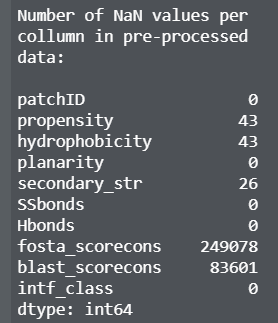
\includegraphics[scale=0.6]{images/nan.png}
  \caption{Αριθμός ελλειπών τιμών}
  \label{fig:nan}
\end{wrapfigure}


Οσον αφορά το τρί\-το ζήτημα, αυτό αποτελεί αρκετά σημαντικό πρόβλημα και πρέπει να αντιμετωπιστεί. Κατά την εκτέλεση των προγραμμάτων που αναφέρθηκαν στην παράγραφο \ref{data}, παρατηρήθηκαν ορισμένες μη έγκυρες τιμές, ο αριθμός των οποίων φαίνεται στην εικόνα. Παρατηρούμε έναν πολύ μεγάλο αριθμό μη έγκυρων τιμών για τα conservation scores χαρακτηριστικά, όπου στο FEP conservation score εχουμε $83,601$ μη έγκυρες τιμές αλλά ειδικότερα στην περίπτωση του homologue conservation score, όπου από τις $317,531$ εγγραφές, οι $249,078$ είναι μη-έγκυρες. Η ύπαρξη τους, παρ' ότι κατανοητή λόγω του τρόπου υπολογισμού των συγκεκριμένων χαρακτηριστικών, δημιουργεί πρόβλημα κατά την εκπαίδευση των μοντέλων, καθώς ένα νευρωνικό δίκτυο δεν μπορεί να τρέξει με μη έγκυρες τιμές ως είσοδο. Για την αντιμετώπιση του συγκεκριμένου προβλήματος δοκιμάστηκαν διάφορες μέθοδοι που θα παρουσιαστούν στη συνέχεια.

\medskip
Στη συνέχεια, πραγματοποιείται μια μορφή κανονικοποίησης των δεδομένων που ονομάζεται \textit{standardization}. Με τον όρο \textit{standardization} ή \textit{Ζ-score normalization} εννοούμε την επεξεργασία των δεδομένων, προκειμένου κάθε χαρακτηριστικό να έχει τις ιδιότητες μιας κανονικής κατανομής, δηλαδή μέση τιμή $0$ και τυπική απόκλιση $1$. Η κανονικοποίηση αυτή είναι αρκετά σημαντική κατά την επεξεργασία τιμών με διαφορετικές κλίμακες, αλλά αποτελεί και προϋπόθεση για πολλούς αλγορίθμους μηχανικής μάθησης. Η κανονικοποίηση αυτή γίνεται με τον ακόλουθο τρόπο, αφαιρώντας από κάθε δείγμα την μέση τιμή του και διαιρώντας με την τυπική του απόκλιση. Αξίζει να δοθεί προσοχή για την κανονικοποίηση ανά χαρακτηριστικό και όχι για όλο το σύνολο των δεδομένων, προκειμένου να έχουμε θετικά αποτελέσματα.

{\Large
\begin{equation} \label{zscore}
    z = \frac{x- \mu_{col}}{\sigma_{col} }
\end{equation}}
where:


{\large
\centering
\begin{conditions}
$\mu_{col}$ & \quad μέση τιμή κάθε χαρακτηριστικού\\
$\sigma_{col}$ & \quad τυπική απόκλιση κάθε χαρακτηριστικού \\
\end{conditions}}


\begin{figure}[h]%
    \centering
    \subfloat[Μέση Τιμή]{{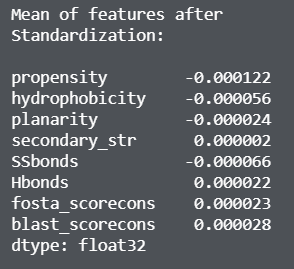
\includegraphics[height=6cm, width=0.45\textwidth]{images/mean.png} }}%
    \hfill
    \subfloat[Τυπική απόκλιση]{{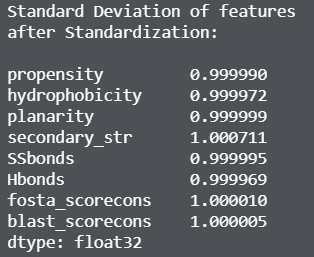
\includegraphics[height=6cm, width=0.45\textwidth]{images/std.png} }}%
    \caption{Standardization}%
    \label{fig:example}%
\end{figure}

\section{Συμπλήρωση μητρώου}

Για την αντιμετώπιση των πολλαπλών \textit{NaN} τιμών που υπήρχαν στα παραδείγματα εκπαίδευσης, χρησιμοποιήθηκε μια τεχνική συμπλήρωσης των τιμών
που ονομάζεται \textit{σημπλήρωση μητρώων} \textit{(matrix completion)}. \textit{Συμπλήρωση μητρώου} ονομάζεται η ανάκτηση ενός πίνακα από υποδειγματολειπτημένες ή ελλειπείς/μη έγκυρες εγγραφές. Ειδικότερα, αν θεωρήσουμε τον επιθυμητό πίνακα ως $X$ και τον πίνακα που περιέχει τις ελλειπείς τιμές ως $X_{\Omega}$, τότε ισχύει η παρακάτω σχέση:

{\Large
\begin{equation}
    X_{\Omega} = H_{\Omega} \odot X + N
\end{equation}}
where:


{
\centering
\begin{conditions}
\Omega & υποσύνολο που περιέχει τις συντεταγμένες των έγκυρων εγγραφών \\
\odot & τελεστής πολ/μού στοιχείο προς στοιχείο\\
\H_{\Omega} & πίνακας δειγματοληψίας \\
N & πίνακας θορύβου \\
\end{conditions}
}

Στην δημοσίευση των \textit{E. J. Candes} και \textit{B. Rectht} \cite{Candes2008}, προτείνεται η ελαχιστοποίηση της τάξης του πίνακα προκειμένου να ανακτηθεί ο αρχικός πίνακας $X$ , δηλαδή:

{\Large
\begin{equation}
    \min_{M} rank(M), \quad s.t \quad M_{\Omega} = X_{\Omega}
\end{equation}}
where:


{\large
\centering
\begin{conditions}
M & πίνακας ανάκτησης, M \in R^{m \times n} \\
X_{\Omega} & H_{\Omega} \odot X\\
M_{\Omega} & προβολή του M στο \Omega \\
\end{conditions}
}

Στην περίπτωση που ο αρχικός πίνακας έχει υποβαθμιστεί από θόρυβο, υπάρχει ανάγκη περιορισμού του επιπέδου θορύβου μέσα σε ένα επιθυμητό εύρος, κάτι που περιγράφεται από την ακόλουθη σχέση:

{\Large
\begin{equation}
    \min_{M} rank(M), \quad s.t \quad \|  M_{\Omega} - X_{\Omega} \|_{F} < \delta
\end{equation}}
where:


{\large
\centering
\begin{conditions}
\| \cdot \|_{F} & Frobenius norm ενός πίνακα \\
$\delta$ & παράμετρος περιορισμού σφάλματος, $\delta$ > 0 \\
\end{conditions}
}

Ωστόσο, το συγκεκριμένο πρόβλημα είναι NP-hard οσον αφορά την επίλυση του, καθώς όλες οι μέθοδοι ακριβούς επίλυσης είναι διπλά εκθετικοί της μέγιστης διάστασης του μητρώου $X$ $\max(m,n)$ όσον αφορά τη διαστασιμότητα. Αυτός είναι και ο λόγος που οι "βέλτιστοι" αλγόριθμοι επιχειρούν να λύσουν προσεγγιστικά το πρόβλημα ελαχιστοποίησης της τάξης (\textit{rank minimization}). Στη συγκεκριμένη εργασία χρησιμοποιήθηκαν δυο τεχνικές συμπλήρωσης μητρώων, με σκοπό την ανάκτηση της πληροφορίας των \textit{NaN} τιμών. Στη συνέχεια αναλύεται η κάθε τεχνική, γίνεται η μαθηματική τους διατύπωση και στο τέλος συγκρίνονται οι δύο τεχνικές σχετικά με την ακρίβειά τους. 


\subsection{Συμπλήρωση μητρώου μέσω SGD}

Η πρώτη τεχνική που χρησιμοποιήθηκε για την συμπλήρωση του dataset βασίζεται στην εργασία των \textit{R. Gemulla}, \textit{P. J. Haas}, \textit{E. Nijkamp} και \textit{Y. Sismanis} με τίτλο \textit{Large-Scale Matrix Factorization with Distributed Stochastic Gradient Descent} \cite{Gemulla2011}. Στη συγκεκριμένη δημοσίευση παρουσιάζεται μια τεχνική παραγοντοποίησης μητρώων μέσω \textit{Stochastic Gradient Descent}.

\medskip
Η μέθοδος gradient descent αποτελεί έναν από τους βασικότερους αλγορίθμους βελτιστοποίησης καθώς και τον πιο διαδεδομένο αλγόριθμο βελτιστοποίησης νευρωνικών δικτύων. Ελαχιστοποιεί μια αντικειμενική συνάρτηση \textbf{$J(\theta)$} με παραμέτρους \textbf{$\theta \in R^{\theta}$} τροποποιώντας τις παραμέτρους στην αντίθετη κατεύθυνση της παραγώγου της αντικειμενικής συνάρτησης \textbf{$\nabla_{\theta} J(\theta)$} συναρτήσει των παραμέτρων. Μια απλή μαθηματική έκφραση των μεθόδων gradient descent είναι η ακόλουθη:

{\Large
\begin{equation}
    \theta_{t} = \theta_{t-1} - n * \nabla_{\theta}J(\theta) 
\end{equation}}
where:


{
\centering
\begin{conditions}
\theta & παράμετροι του μοντέλου. \\
J(\theta) & αντικειμενική συνάρτηση. \\
n & ρυθμός μάθησης (learning rate). \\
\end{conditions}
}

\medskip
Ωστόσο, καθώς για τον υπολογισμό ενός μόνο βήματος τροποποίησης των παραμέτρων απαιτείται η εύρεση της παραγώγου ολόκληρου του σετ δεδομένων, οι αλγόριθμοι gradient descent τείνουν να συγκλίνουν πολύ αργά και να δημιουργούν προβλήματα για την βελτιστοποίηση δεδομένων που δεν χωρούν στη μνήμη. Για το λόγο αυτό προτάθηκε η μέθοδος \textit{Stochastic Gradient Descent}, που αποτελεί τροποποίηση της μεθόδου gradient descent. Αντικαθιστά τον υπολογισμό της παραγώγου ολόκληρου του σετ των δεδομένων με μια \textit{προσέγγιση} αυτής, υπολογισμένη από ένα τυχαίο υποσύνολου των δεδομένων. 

Ενώ η μέθοδος gradient descent συγκλίνει σε ένα τοπικό ελάχιστο, η μεγάλη διακύμανση με την οποία συγκλίνει η μέθοδος Stochastic Gradient Descent επιτρέπει τη σύγκλιση σε νέα και πιθανώς βελτιωμένα τοπικά ελάχιστα. Απο την άλλη, η έντονη αυτή διακύμανση καθιστά τη διαδικασία σύγκλισης (λόγω άλματων στις τιμές της αντικειμενικής συνάρτησης). Για την αντιμετώπιση αυτού του προβλήματος, χρησιμοποιείται μειούμενος ρυθμός μάθησης και παρατηρείται παρόμοιος ρυθμός σύγκλισης με αυτόν της gradient descent.

\medskip
\begin{figure}[h]
  \centering
  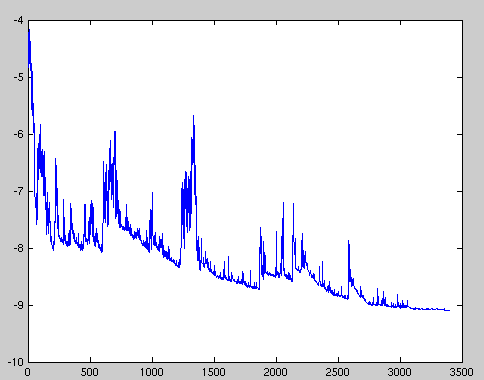
\includegraphics[scale=0.75]{images/Stogra.png}
  \caption{Διακύμανση SGD}
  \label{fig:StoGra}
\end{figure}

\medskip
Η μαθηματική διατύπωση της Stochastic Gradient Descent, όπου πραγματοποιείται τροποποίηση των παραμέτρων με βάση ένα τυχαίο υποσύνολο των δεδομένων $x^{(i)}, y^{(i)}$ είναι η εξής:

{\Large
\begin{equation}
    \theta_{t} = \theta_{t-1} - n * \nabla_{\theta}J(\theta ; x^{(i)} ; y^{(i)}) 
\end{equation}}
where:


{
\centering
\begin{conditions}
\theta & παράμετροι του μοντέλου. \\
J(\theta) & αντικειμενική συνάρτηση. \\
n & ρυθμός μάθησης (learning rate). \\
\end{conditions}
}

\medskip
Για την εφαρμογή της μεθόδου Stochastic Gradient Descent στην παραγοντοποίηση του συνόλου δεδομένων μας, θεωρούμε ως παραμέτρους $θ$ τα μητρώα $W$ και $H$ (τέτοια ώστε $V = WH$ οπου $V$ το αρχικό σύνολο των δεδομένων μας). Ακόμη, θεωρούμε ως αντικειμενική συνάρτηση τη συνάρτηση απωλειών $L_{NZSL}$, που ορίζεται ως εξής: 

{\Large
\begin{equation}
    L_{NZSL} = \sum_{i,j :\; V_{ij} \neq 0} \; (V_{ij} - [WH]_{ij})^2
\end{equation}}

Παράλληλα, αναλύουμε την $L_{NZSL}$ ως άθροισμα συναρτήσεων τοπικών απωλειών $l$ σε ένα υποσύνολο των δεδομένων $V$, δηλαδή: 

{\Large
\begin{equation}
    L = \sum_{i,j \in \mathbb{Z}} \; l(V_{ij} , W_{i*}, H_{*j})
\end{equation}}

Ο αλγόριθμος που χρησιμοποιήθηκε με χρήση Stochastic Gradient Descent για την παραγοντοποίηση του μητρώου δεδομένων μας είναι ο εξής:

\medskip
\begin{algorithm}[H]
\SetAlgoLined
\DontPrintSemicolon
\KwData{\\$Z$: σύνολο δεδομένων, \\$W,H$: αρχικοποιημένοι με τυχαίες τιμές.}
\While{δεν συγκλίνει}{
    Επιλογή τυχαίου παραδείγματος $(i,j) \in Z$. \;
    \Large  $W^{'}_{i*} \leftarrow W_{i*} - \epsilon_{n} \frac{\partial}{\partial W_{i*}} l(V_{ij} , W_{i*}, H_{*j})$ \;
    $H^{'}_{*j} \leftarrow H_{*j} - \epsilon_{n} \frac{\partial}{\partial H_{*j}} l(V_{ij} , W_{i*}, H_{*j})$ \;
    $W_{i*} \leftarrow W^{'}_{i*}$ \;
    $H_{*j} \leftarrow H^{'}_{*j}$ \;
}
\caption{SGD for Matrix Factorization \label{SGDMF}}
\end{algorithm}

\bigskip
Mετά την επιλογή του τυχαίου παραδείγματος $(i,j) \in Z$, χρειάζεται μόνο η τροποποίηση των $W_{i*}$ και $H_{*j}$, μειώνοντας σημαντικά τους αναγκαίους υπολογισμούς. Η μείωση αυτή οφείλεται και στην έκφραση των συνολικών απωλειών ως άθροισμα τοπικών απωλειών. Όσον αφορά την αντικατάσταση της ακριβούς παραγώγου με την προσέγγισή της, εκτός απο την μείωση της υπολογιστικής πολυπλοκότητας, διευκολύνεται η αποφυγή τοπικών ελαχίστων, εντοπίζεται επαναληψιμότητα σε δεδομένα ενώ παράλληλα οι τροποποιήσεις βασισμένες σε δεδομένα συγκεκριμένων γραμμών/στηλών μειώνει τις απώλειες σε αντίστοιχες γραμμές/στήλες. Επομένως, όσο μεγαλύτερη ομοιότητα εμφανίζεται στα δεδομένα, τόσο ταχύτερη είναι η σύγκλιση του αλγορίθμου \cite{Bottou2007}. Στην περίπτωση του dataset μας, καθώς κάθε αλληλεπίδραση χωρίζεται σε patches που διαθέτουν παρόμοιες (αν όχι πανομοιότυπες) ιδιότητες, παρατηρούνται πολλαπλές όμοιες εγγραφές, με αποτέλεσμα την γρήγορη σύγκλιση του αλγορίθμου. Με απλές αλγεβρικές τροποποιήσεις προκύπτουν και οι παράγωγοι της αντικειμενικής συνάρτησης $L_{NZSL}$ ως:

\bigskip
\begingroup
\centering
\newcommand\T{\rule{0pt}{2.6ex}} % Top strut
\newcommand\B{\rule[-1.2ex]{0pt}{0pt}} % Bottom strut
\begin{tabularx}{\textwidth} { 
  | >{\centering\arraybackslash}X 
  |  }
 \hline
 \textbf{Συνάρτηση Απώλειας - Ορισμός και Παράγωγοι }\T\B  \\
 \hline
 \LARGE $ L_{NZSL} = \sum_{(i,j) \in Z} \; (V_{ij} - [WH]_{ij})^2$ \T\B \\
 \LARGE $\frac{\partial}{\partial W_{ik}} L_{ij} = -2*(V_{ij} - [WH]_{ij})*H_{kj}$ \T\B \\
 \LARGE $\frac{\partial}{\partial H_{kj}} L_{ij} = -2*(V_{ij} - [WH]_{ij})*W_{ik}$ \T\B \\
 \hline
\end{tabularx}
\captionof{table}{Συνάρτηση Απώλειας - Ορισμός,Παράγωγοι} 
\label{Συνάρτηση Απώλειας - Ορισμός και Παράγωγοι}
\endgroup

\medskip
Για την υλοποίηση του αλγορίθμου \ref{SGDMF}, χρησιμοποιήθηκε το υπολογιστικό περιβάλλον της Matlab και για \textit{ρυθμό εκπαίδευσης} χρησιμοποιήθηκε ως αρχική τιμή το $2^{-27}$ (που αποτελούσε τη μέγιστη τιμή θετική τιμή για την οποία δεν απέκλεινε ο αλγόριθμος στα πρώτα βήματα) ενώ στη συνέχεια χρησιμοποιήθηκε μια ευρετική μέθοδος που ονομάζεται \textbf{bold driver} και χρησιμοποιείται συχνά για την τροποποίηση του βήματος μεθόδων gradient descent. Ειδικότερα, σε κάθε εποχή αυξάνεται ο ρυθμός εκπαίδευσης κατά ένα μικρό ποσοστό (στην περίπτωσή μας $5\%$) εφόσον παρατηρήθεί μείωση στις απώλειες, ενώ σε περίπτωση αύξησης των απωλειών μειώνεται δραστικά ο ρυθμός εκπαίδευσης (π.χ. $50\%$). Τέλος, κατά τη διάρκεια κάθε εποχής ο ρυθμός εκπαίδευσης παραμένει σταθερός. Όσον αφορά τη σύγκλιση του αλγορίθμου, χρησιμοποιήθηκε ως αντικειμενική συνάρτηση η σχετική απόσταση μεταξύ των γνωστών (μη-μηδενικών) στοιχείων του αρχικού συνόλου δεδομένων και των αντίστοιχων στοιχείων του μητρώου που υπολογίστηκε ($WH$).


Στη συνέχεια, πραγματοποιήθηκαν πειράματα προκειμένου να βρεθεί η τάξη της βέλτιστης αναπαράστασης χαμηλότερης τάξης του αρχικού μας συνόλου δεδομένων και παρακάτω παρουσιάζονται τα αποτελέσματα. Παρατηρούμε ότι η μέθοδος συγκλίνει αρκετά γρήγορα, ενώ όσο αυξάνεται η τάξη του ανακατασκετασμένου πίνακα μειώνονται σημαντικά οι σχετικές απώλειες. Για τάξη $r=8$ παρατηρήθηκαν οι ελάχιστες σχετικές απώλειες $Loss = 0.16255$. Πειράματα που διεξήχθησαν και για τάξεις με $ r > 8$ δεν έδειξαν σημαντική βελτίωση, οπότε χρησιμοποιήθηκε η συγκεκριμένη ανακατασκευή για την εκπαίδευση των νευρωνικών μοντέλων.

\medskip
\begin{figure}[H]
  \centering
  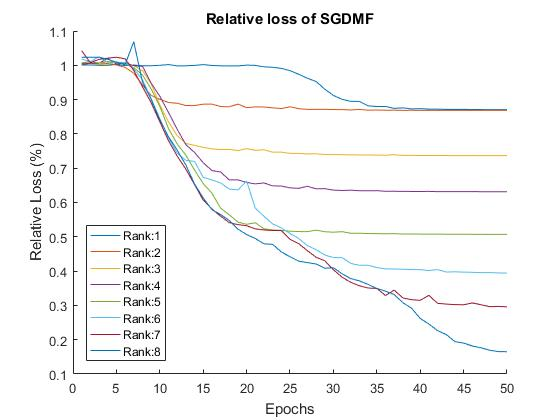
\includegraphics[width=\textwidth]{images/SGDMFlosssmall.jpg}
  \caption{Σχετικές απώλειες SGD}
  \label{fig:SGDMFlosssmall}
\end{figure}


\medskip
\subsection{Παραγοντοποίηση μητρώου μέσω τανυστικής αποδόμησης}

Στο χώρο της μηχανικής μάθησης, ένας \textit{τανυστής} (\textit{tensor}) ονομάζεται μια πολυδιάστατη δομή ή ,πιο αυστηρά, ένας τανυστής $N$-οστής τάξης είναι το αποτέλεσμα του τανυστικού γινομένου $N$ διανυσματικών χώρων, ο καθένας εκ των οποίων έχει το δικό του σύστημα συντεταγμένων \cite{Kolda2009}. Προτού περάσουμε στην παρουσίαση της μεθόδου που χρησιμοποιήθηκε για την παραγοντοποίηση μητρώου μέσω τανυστικής αποδόμησης, θα οριστούν κάποιες βασικές έννοιες σχετικά με τους τανυστές. Ως \textit{τάξη} (\textit{order}) ενός τανυστή ορίζουμε τη διαστασιμότητά του. Στη συγκεκριμένη διπλωματική εργασία, οι τανυστές με τους οποίους εργαζόμαστε είναι δεύτερης τάξης και αποτελούν μητρώα, επομένως μελλοντικές αναφορές στον όρο "τανυστής" θα απασχολούν τανυστές $2^{ης}$ τάξης για λόγους απλότητας, ενώ ο συμβολισμός των τανυστών δεύτερης τάξης θα γίνεται με κεφαλαία γράμματα με έντονη γραφή (π.χ. $\textbf{A}$). Τα στοιχεία $(i,j)$ ενός τανυστή $\textbf{A}$ συμβολίζονται ως $a_{ij}$ και έχουν δείκτες $i = 1, ... , I$. Ως νόρμα ενός τανυστή {\Large $\textbf{A} \in \mathbb{R}^{I \times J }$ } ορίζεται η τετραγωνική ρίζα του αθροίσματος των τετραγώνων όλων των στοιχείων του, δηλαδη:


{\Large\begin{equation}
    \| \textbf{A} \| = \sqrt{\sum_{i=1}^{I}\sum_{j=1}^{J} a_{ij}^2}
\end{equation}}

Ιδιαίτερη σημασία στην ανάλυση τανυστών στη μηχανική μάθηση εμφανίζουν και τα γινόμενα μητρώων, προκειμένου να εκφραστεί ένας τανυστής ως το προϊόν αυτών. Μερικά από αυτά τα γινόμενα είναι το γινόμενο \textit{Kronecker}, το γινόμενο \textit{Khatri-Rao}, το γινόμενο \textit{Hadamard}, με εκτενή ανάλυση αυτών στη σχετική βιβλιογραφία \cite{Liu2008}. 

\medskip
Ως εισαγωγή στην αποδόμηση τανυστών, πρέπει να ορίσουμε την έννοια του βαθμού ενός τανυστή. Ένας τανυστής $N$-οστής τάξης θεωρείται \textit{πρώτου βαθμού} (\textit{rank one}) όταν μπορεί να γραφεί ως το εξωτερικό γινόμενο $N$ διανυσμάτων, π.χ: $\large{\textbf{A} = a^{(1)} \circ a^{(2)}}$, οπου το $\large{\circ}$ συμβολίζει το εξωτερικό γινόμενο διανυσμάτων. Ο \textit{βαθμός} (\textit{rank}) ενός τανυστή \textbf{A} ορίζεται ως ο ελάχιστος αριθμός τανυστών πρώτου βαθμού που το άθροισμα αυτών μας δίνει τον \textbf{A}. Η ιδέα της έκφρασης ενός τανυστή ως το πεπερασμένο άθροισμα τανυστών πρώτου βαθμού παρουσιάστηκε το 1927 από τον \textit{F. Hitchcock} ως πολυαδική μορφή ενός τανυστή \cite{Hitchcock1927}, ενώ το 1944 o \textit{R. Cattell} παρουσίασε ιδέες για παράλληλη ανάλυση πολυαδικών μορφών και χρήση πολλαπλών αξόνων για ανάλυση \cite{Cattell1944}. Οι έννοιες αυτές έμειναν σχετικά άγνωστες μέχρι το 1970 και την εισαγωγή τους στο χώρο της ψυχοακουστικής, με τη μορφή των \textit{CANDECOMP (Canonical Decompostion)} από τους \textit{J. D. Carroll} και \textit{J. J. Chang} \cite{Carroll1970} και \textit{PARAFAC (Parallel Factors)} από τον \textit{R. Harshman} \cite{harshman1972}. Θα αναφερόμαστε στην αποδόμηση τανυστών CANDECOMP/PARAFAC ως \textit{αποδόμηση CP} (\textit{CP decomposition}). Η αποδόμηση CP παραγοντοποιεί έναν τανυστή ως ένα άθροισμα R τανυστών πρώτου βαθμού \cite{Papastergiou2019} \cite{Papastergiou2018}. Για π.χ., δοσμένου ενός τανυστή τρίτης τάξης $\textit{\textbf{X}} \in \mathbb{R}^{I \times J \times K}$, επιθυμούμε να τον γράψουμε ως: 

{\Large
\begin{equation}
    \textit{\textbf{X}} \approx \sum_{r=1}^{R}a_r \circ b_r \circ c_r
\end{equation}}
οπου: R θετικός ακέραιος, $a_r \in \mathbb{R}^I$, $b_r \in \mathbb{R}^J$ και $c_r \in \mathbb{R}^K$ για \newline$r = 1,...,R$. Στην εικόνα \ref{fig:CP} παρουσιάζεται η CP αποδόμηση ενός τανυστή τρίτης τάξης.

\medskip
\begin{figure}[h]
  \centering
  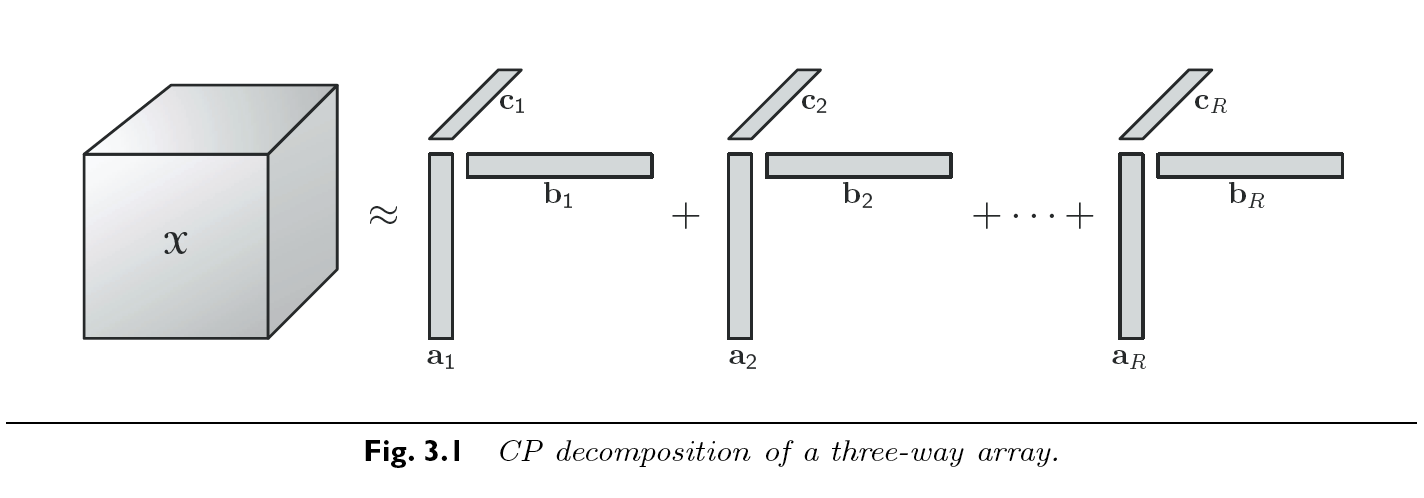
\includegraphics[scale=0.5]{images/CP.png}
  \caption{Αποδόμηση τανυστή τρίτης τάξης}
  \label{fig:CP}
\end{figure}

\medskip
Το ζητούμενο στην τανυστική αποδόμηση είναι η εύρεση του αριθμού R των διανυσμάτων που προσεγγίζουν τον τανυστή. Συνεπώς, σύμφωνα με τους παραπάνω ορισμούς, το R είναι ο βαθμός του τανυστή και η διαδικασία εύρεσής του είναι μια αρκετά πολύπλοκη διαδικασία ( εχει αποδειχθεί ότι είναι NP-hard πρόβλημα \cite{Håstad2006} ). Πρακτικά, η εύρεση της τάξης R ενός τανυστή γίνεται εφαρμόζοντας διαφορετικές τιμές στο R και βλέποντας πόσο καλά προσεγγίζεται ο αρχικός τανυστής από τον ανακατασκευασμένο.Η μαθηματική έκφραση της παραπάνω πρότασης παρουσιάζεται στην εξίσωση \ref{cpr}, όπου με λ συμβολίζουμε ένα διάνυσμα στο οποίο αποθηκεύονται τα βάρη και το οποίο πολλαπλασιάζουμε με το εξωτερικό γινόμενο των τριών διανυσμάτων. 

{\Large
\begin{equation}\label{cpr}
    \min_{\widehat{X}} \| X - \widehat{X} \| \; where \; \widehat{X} = \sum_{r=1}^{R} \lambda_{r} \, a_r \circ b_r \circ c_r
\end{equation}}

Στη διπλωματική εργασία χρησιμοποιήθηκε μια τροποποιημένη εκδοχή της αποδόμησης CP που ονομάζεται \textit{βεβαρημένη βελτιστοποίηση μεσω CP αποδόμησης } (\textit{CP Weighted Optimization} η πίο απλά \textit{CP-WOPT}) \cite{Acar_2011} \cite{Papastergiou2017}. Ειδικότερα, στην περίπτωση τανυστών με ελλιπή δεδομένα, η αποδόμηση CP μπορεί να μοντελοποιηθεί ως ένα βεβαρημένο πρόβλημα ελαχίστων τετραγώνων με έμφαση μόνο στις γνωστές τιμές. Η μέθοδος CP-WOPT επιλύει το βεβαρημένο πρόβλημα ελαχίστων τετραγώνων με τη χρήση βελτιστοποίησης πρώτης τάξης. Τροποποιεί την συνάρτηση σφάλματος ωστε να αγνοούνται οι μη υπάρχουσες τιμές και να μοντελοποιούνται μονάχα οι γνωστές τιμές, επομένως μετά μπορούν να χρησιμοποιηθούν μέθοδοι μη γραμμικής βελτιστοποίησης για την απευθείας επίλυση του βεβαρημένου προβλήματος ελαχίστων τετραγώνων με CP αποδόμηση. Η τροποποίηση της συνάρτησης σφάλματος φαίνεται στην εξίσωση \ref{CPWOPT}:

{\Large
\begin{equation}\label{CPWOPT}
    \textit{f}_w(A,B)= \frac{1}{2}\sum_{i=1}^{I}\sum_{j=1}^{J}\{ w_{ij} ( x_{ij} - \sum_{r=1}^R a_{ir} b_{jr} )\}^{2}
\end{equation}
}
οπου \textbf{W} ενας μη-αρνητικός τανυστής βαρών ίδιου μεγέθους με τον \textbf{X} που τα στοιχεία του ορίζονται ως:

{\Large 
\begin{equation}
w_{ij} = 
\begin{cases}
1 & if \; $x_{ij}$ is known. \\
0 & if \; $x_{ij}$ is missing. \\
\end{cases}
\end{equation}}


\medskip
Πρακτικά ο τανυστής \textbf{W} λειτουργεί ως μάσκα προκειμένου να ληφθούν υπόψη μόνο οι γνωστές τιμές. Χρησιμοποιώντας τους ορισμούς που παρουσιάστηκαν προηγουμένως, μπορούμε να ορίσουμε τη συνάρτηση απωλειών ως:

{\Large
\begin{equation} \label{CPWOPT2}
    \textit{f}_{w}(\textbf{A},\textbf{B}) = \frac{1}{2} \|\textbf{W}. * (\textbf{X} - \textbf{AB}^{T}) \|^{2}
\end{equation}
}
όπου * ο τελεστής του γινομένου \textit{Hadamard} (ή αλλιώς το γινόμενό τους στοιχείο προς στοιχείο). Σκοπός η εύρεση των \textbf{A} και \textbf{B} που ελαχιστοποιούν την αντικειμενική συνάρτηση \ref{CPWOPT2}. 

Για την ελαχιστοποίηση της αντικειμενικής συνάρτησης χρησιμοποιήθηκε ως αλγόριθμος βελτιστοποίησης η μέθοδος \textit{μη γραμμικής συζυγούς παραγώγου} (\textit{Nonlinear conjugate gradient method - ncg}) \cite{Sanmatias1998}. Πρόκειται για μια μέθοδο που επεκτείνεται ικανοποιητικά για προβλήματα μεγάλου μεγέθους και έχει την ακόλουθη έκφραση:
 
 Δεδομένου ενός προβλήματος ελαχιστοποίησης χωρίς περιορισμούς {\large $\min \textit{f}(x), x \in \mathbb{R}^{n}$}, η μέθοδος \textit{ncg} έχει τη μορφή:
{\Large
\begin{equation}
    x_{k+1} = x_k + a_k d_k, \; k=0,1,2,...
\end{equation}
}
όπου
{\large
\begin{conditions}
$x_0$ & αρχικό σημείο εκκίνησης.\\
$a_k$ & ρυθμός εκπαίδευσης (learing rate).\\
$d_k$ & \begin{cases}
$-g_k$ & k=0; \\
$-g_k + \beta_{k} d_{k-1}$ & $k \geq 1$, \\
\end{cases} 
where $g_k = \nabla\textit{f}(x_{k})$
\end{conditions}
}
Διαφορετικά $β_k$ ορίζουν διαφορετικές μεθόδους \textit{ncg}. Μερικοι δημοφιλείς τύποι για το $β_k$ παρουσιάζονται στον πίνακα \ref{beta}

{\large
\medskip
\begingroup
\centering
\newcommand\T{\rule{0pt}{3.0ex}} % Top strut
\newcommand\B{\rule[-2.0ex]{0pt}{0pt}} % Bottom strut
\begin{tabularx}{0.8\textwidth} { 
  | >{\raggedright\arraybackslash}X 
  | >{\centering\arraybackslash}X 
  | >{\raggedright\arraybackslash}X | }
 \hline
 \multicolumn{2}{|c|}{\textbf{Τύποι $\beta_k$ για μεθόδους ncg}} \T\B \\
 \hline
 \textbf{Μέθοδος}\T\B & \textbf{Τύπος}\T\B \\
 \hline
 \textit{Fletcher-Reeves}\T\B & {\LARGE $\beta^{FR} = \frac{\| g_k \|^{2}}{\| g_{k-1} \|^{2}} $\T\B} \\
 \hline
 \textit{Polak-Ribiere-Polyak}\T\B & {\LARGE $\beta^{PRP} = \frac{g_{k}^{\textit{T}}(g_{k} - g_{k-1}) }{\| g_{k-1} \|^{2}} $\T\B} \\
 \hline
 \textit{Hestenes-Stiefiel}\T\B & {\LARGE $\beta^{HS} = \frac{g_{k}^{\textit{T}}(g_{k} - g_{k-1}) }{d_{k-1}^{\textit{T}}(g_{k} - g_{k-1})} $\T\B} \\
 \hline
 \textit{Conjugate Descent}\T\B & {\LARGE $\beta^{CD} = - \frac{\| g_k \|^{2}}{d_{k-1}^{\textit{T}} g_{k-1}} $\T\B} \\
 \hline
 \textit{Dai-Yuan}\T\B & {\LARGE $\beta^{DY} = \frac{\| g_k \|^{2}}{d_{k-1}^{\textit{T}}(g_{k} - g_{k-1})} $\T\B} \\
 \hline
 \textit{Liu-Storey}\T\B & {\LARGE $\beta^{LS} = - \frac{g_{k}^{\textit{T}}(g_{k} - g_{k-1}}{d_{k-1}^{\textit{T}} g_{k-1}} $\T\B} \\
 \hline
\end{tabularx}
\captionof{table}{Δημοφιλείς τύποι $\beta_k$ \cite{SHI2008}} 
\label{beta}
\endgroup}


\medskip
\begin{figure}[h]
  \centering
  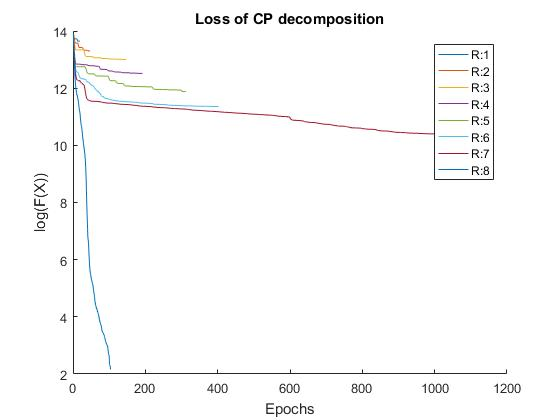
\includegraphics[scale=0.57]{images/CPdecomp.jpg}
  \caption{Απώλειες CP αποδόμησης}
  \label{fig:CPdecomp}
\end{figure}

\medskip
Στα πλαίσια της διπλωματικής χρησιμοποιήθηκε ο τύπος των \textit{Polak-Ribiere-Polyak} για την τροποποίηση του $\beta_k$. Στην εικόνα \ref{fig:CPdecomp} παρουσιάζονται οπτικά τα αποτελέσματα της CP αποδόμησης για διαφορετικούς βαθμούς r, με τις απώλειες εμφανίζονται λογαριθμικά λόγω της τεράστιας διαφοράς των τιμών. Παρατηρούμε ότι για $r=8$ ο ανακατασκευασμένος τανυστής προσεγγίζει σημαντικά τον αρχικό τανυστή ($F(x)=8.75$), επομένως λαμβάνουμε τη συγκεκριμένη ανακατασκευή ως σύνολο δεδομένων προς εκπαίδευση.

\bigskip
\section{Εκπαίδευση}

Έπειτα από την ανακατασκευή των δεδομένων με τις μεθόδους της παραγοντοποίησης μητρώου μέσω SGD και της τανυστικής αποδόμησης, τα δεδομένα είναι σε κατάλληλη μορφή για να τροφοδοτηθούν σε νευρωνικά δίκτυα. Για τη σωστή αντιμετώπιση του προβλήματος, πρέπει να επιλεγεί τόσο η κατάλληλη \textit{δομή/αρχιτεκτονική} νευρωνικών δικτύων, αλλά και να γίνει σωστή ρύθμιση των υπερπαραμέτρων, στις οποίες έγινε αναφορά στο κεφάλαιο \ref{ch:chap2}. Η κατασκευή των νευρωνικών δικτύων καθορίζει τον τρόπο μη γραμμικής συσχέτισης μεταξύ εισόδων και εξόδου. Δοκιμάστηκαν πολλές διαφορετικές αρχιτεκτονικές και ρυθμίστηκε πειραματικά μια πληθώρα παραμέτρων, ωστόσο στα πλαίσια της εργασίας θα παρουσιαστούν οι δύο καλύτερες αρχιτεκτονικές, μια αρχιτεκτονική \textit{πλήρως διασυνδεδεμένου δικτύου} (\textit{fully connected neural network}) και μια αρχιτεκτονική \textit{συνελικτικού δικτύου} (\textit{convolutional neural network}).
\medskip
Αρχικά, η εκπαίδευση καθώς και η αξιολόγηση των δεδομένων πραγματοποιήθηκε με τη μέθοδο \textit{k-απλή επικυρωμένη διαστάυρωση} \textit{k-fold cross-validation}.\textit{Επικυρωμένη διασταύρωση} (\textit{Cross-validation}) ονομάζεται μια στατιστική μέθοδος που χρησιμοποιείται για την εκτίμιση της ικανότητας των νευρωνικών δικτύων. Στην περίπτωση του k-fold cross validation, τα δεδομένα χωρίζονται σε $k$ ομάδες, με τις $k-1$ να αποτελούν το σετ δεδομένων εκπαίδευσης (training set) και την 1 να αποτελεί το σετ δεδομένων αξιολόγησης (test set). Το μοντέλο εκπαιδεύεται με τα δεδομένα εκπαίδευσης, αξιολογείται η απόδοση του στα δεδομένα αξιολόγησης και αποθηκεύονται οι μετρικές αξιολόγησης. Η διαδικασία επαναλαμβάνεται για κάθε μια εκ των $k$ ομάδων και η απόδοση του μοντέλου ορίζεται ως ο μέσος όρος των αποδόσεων για κάθε εκπαίδευση του μοντέλου. Στην περίπτωσή μας, επιλέχθηκε η αξιολόγηση των μοντέλων μέσω 10-fold cross validation, προκειμένου τα αποτελέσματα να είναι συγκρίσιμα με τα αποτελέσματα της δημοσίευσης \cite{Northey2017}.

\medskip
\begin{figure}[h]
  \centering
  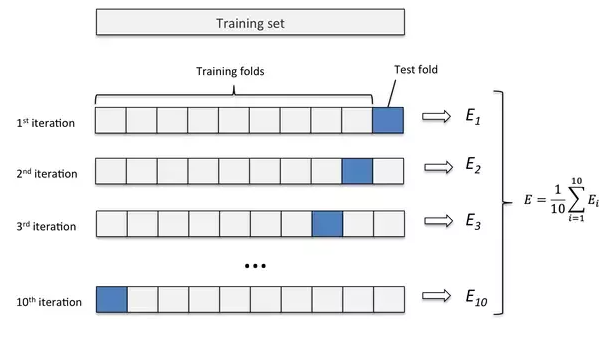
\includegraphics[scale=0.8]{images/crossval.png}
  \caption{10-fold cross validation}
  \label{fig:crossval}
\end{figure}

\subsection{Πλήρως διασυνδεδεμένη αρχιτεκτονική}

Η πρώτη αρχιτεκτονική που χρησιμοποιήθηκε, καθώς εμφανίζεται γενικότερα στην σχετική βιβλιογραφία και έχει χρησιμοποιηθεί με επιτυχία στο παρελθόν σε αντίστοιχα προβλήματα υπολογιστικής βιολογίας, είναι αυτή του πλήρως διασυνδεδεμένου νευρωνικού δικτύου. Ύστερα από πολλαπλά πειράματα, η "βέλτιστη" αρχιτεκτονική αποτελείται:

\begin{itemize}
    \item ένα επίπεδο εισόδου με $1024$ νευρώνες,
    \item τέσσερα κρυφά επίπεδα με $512,264,128,64$ νευρώνες αντίστοιχα και
    \item ένα επίπεδο εξόδου με $2$ νευρώνες.
\end{itemize}

\medskip
Ως συνάρτηση ενεργοποίησης, για το επίπεδο εισόδου και τα τέσσερα κρυφά επίπεδα χρησιμοποιήθηκε η \textit{ReLu}, ενώ για το επίπεδο εξόδου καθώς το πρόβλημα μας είναι κατηγοριοποίηση δυαδικής μορφής ( \textit{binary classification} ), χρησιμοποιήθηκε η σιγμοειδής συνάρτηση (\textit{sigmoid}). Κατά την εκπαίδευση χρησιμοποιήθηκε ως βελτιστοποιητής ο \textit{Adam} (\textit{Adaptive Moment Estimation}) με ρυθμό εκπαίδευσης $\textit{L}_r = 0.0001$. Ακόμη, δοκιμάστηκε η προσθήκη επιπέδων \textit{απόρριψης} (\textit{dropout layers}). Η λειτουργία των επιπέδων απόρριψης συνοψίζεται στην απενεργοποίηση νευρώνων του προηγούμενου επιπέδου, με τον αριθμό των απενεργοποιημένων νευρώνων σε κάθε εποχή να ορίζεται από μια υπερπαράμετρο που ονομάζεται \textit{ρυθμός απόρριψης} (\textit{Dropout rate}). Το επίπεδο απόρριψης εφαρμόζεται για να αποφευχθεί το φαινόμενο του \textit{υπερταιριάσματος} (\textit{overfitting}), κατά το οποίο το νευρωνικό "απομνημονεύει" τα δεδομένα εκπαίδευσης έχοντας εξαιρετική απόδοση σε αυτά αλλά έχει χαμηλή απόδοση σε νέα, "άγνωστα" δεδομένα. Ωστόσο, στην περίπτωση μας η προσθήκη επιπέδων απόρριψης δεν βοήθησε, γεγονός που αποδίδεται στον μικρό αριθμός χαρακτηριστικών ( 8 χαρακτηριστικά) των δεδομένων εκπαίδευσης.     

\tikzset{%
  every neuron/.style={
    circle,
    draw,
    minimum size=1cm
  },
  neuron missing/.style={
    draw=none, 
    scale=4,
    text height=0.333cm,
    execute at begin node=\color{black}$\vdots$
  },
}

\begin{figure}[h]
\centering
\begin{tikzpicture}[x=1.5cm, y=1.5cm, >=stealth]

\foreach \m/\l [count=\y] in {1,2,3,missing,4}
  \node [every neuron/.try, neuron \m/.try] (input-\m) at (0,2.5-\y) {};

\foreach \m [count=\y] in {1,missing,2}
  \node [every neuron/.try, neuron \m/.try ] (1-hidden-\m) at (1.25,2-\y*1.25) {};

\foreach \m [count=\y] in {1,missing,2}
  \node [every neuron/.try, neuron \m/.try ] (2-hidden-\m) at (2.5,2-\y*1.25) {};
  
 \foreach \m [count=\y] in {1,missing,2}
  \node [every neuron/.try, neuron \m/.try ] (3-hidden-\m) at (3.75,2-\y*1.25) {};

\foreach \m [count=\y] in {1,missing,2}
  \node [every neuron/.try, neuron \m/.try ] (4-hidden-\m) at (5,2-\y*1.25) {};
  
  
\foreach \m [count=\y] in {1,2}
  \node [every neuron/.try, neuron \m/.try ] (output-\m) at (6.35,2-\y*1.7) {};

\foreach \l [count=\i] in {1,2,3,n}
  \draw [<-] (input-\i) -- ++(-1,0)
    node [above, midway] {$I_\l$};

\foreach \l [count=\i] in {1,512}
  \node [below] at (1-hidden-\i.south) {$H_{\l}$};
  
  \foreach \l [count=\i] in {1,264}
  \node [below] at (2-hidden-\i.south) {$H_{\l}$};

\foreach \l [count=\i] in {1,128}
  \node [below] at (3-hidden-\i.south) {$H_{\l}$};

\foreach \l [count=\i] in {1,64}
  \node [below] at (4-hidden-\i.south) {$H_{\l}$};
  
\foreach \l [count=\i] in {1,...,2}
  \draw [->] (output-\i) -- ++(1,0)
    node [above, midway] {$O_\l$};

\foreach \i in {1,...,4}
  \foreach \j in {1,...,2}
    \draw [->] (input-\i) -- (1-hidden-\j);

\foreach \i in {1,...,2}
  \foreach \j in {1,...,2}
    \draw [->] (1-hidden-\i) -- (2-hidden-\j);

\foreach \i in {1,...,2}
  \foreach \j in {1,...,2}
    \draw [->] (2-hidden-\i) -- (3-hidden-\j);

\foreach \i in {1,...,2}
  \foreach \j in {1,...,2}
    \draw [->] (3-hidden-\i) -- (4-hidden-\j);

    
\foreach \i in {1,...,2}
  \foreach \j in {1,...,2}
    \draw [->] (4-hidden-\i) -- (output-\j);

\foreach \l [count=\x from 0] in {Input\\Layer, Hidden\\Layer 1, Hidden\\Layer 2, Hidden\\Layer 3, Hidden\\Layer 4, Ouput\\Layer}
  \node [align=center, above] at (\x*1.25,2) {\l};

\end{tikzpicture}
\caption{Fully connected αρχιτεκτονική}
\label{fig:FC_Arch}
\end{figure}


\bigskip
\subsection{Συνελικτική αρχιτεκτονική}

Υστερα από τα πειράματα που πραγματοποιήθηκαν σε πλήρως διασυνδεδεμένες αρχιτεκτονικές, ακολούθησε η δημιουργία και ο πειραματισμός με συνελικτικές δομές νευρωνικών δικτύων. Τα συνελικτικά νευρωνικά δίκτυα έχουν αναπτυχθεί σημαντικά τα τελευταία χρόνια λόγω της ικανότητάς τους να αναλύουν χωρική πληροφορία. Όσον αφορά την αρχιτεκτονική του συνελικτικού δικτύου, αποτελείται από 6 $1-D$ συνελικτικά επίπεδα με $32,32,64,64,128,128$ φίλτρα αντίστοιχα, με συνάρτηση ενεργοποίησης ReLu, όπου κάθε φίλτρο αποτελείται από ένα παράθυρο $3 \times 3$ , με κάθε συνελικτικό φίλτρο να ακολουθείται από ένα επίπεδο υποδειγματοληψίας που ονομάζεται \textit{Max Pooling}, με μέγεθος παραθύρου $3 \times 3$. 

\medskip
\begin{figure}[h]
  \centering
  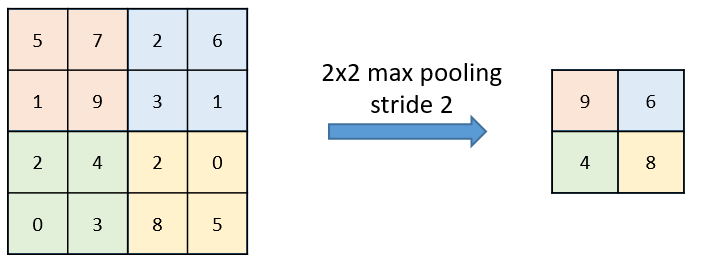
\includegraphics[scale=0.65]{images/maxpool.png}
  \caption{Max Pooling}
  \label{fig:maxpool}
\end{figure}

\medskip
Κατά τη διαδικασία max pooling, από κάθε παράθυρο επιλέγεται η μέγιστη τιμή ως τιμη ως τιμή αντιπρόσωπος για το επόμενο επίπεδο. Με αυτό τον τρόπο επιτυγχάνεται μείωση της διαστασιμότητας του δικτύου ενώ παράλληλα πραγματοποιείται περιορισμός του θορύβου, καθώς οι θορυβώδεις τιμές απορρίπτονται. Στο τέλος του 6ου συνελικτικού επιπέδου εντοπίζεται ένα επίπεδο εξομάλυνσης (\textit{flatten layer}), που μετατρέπει την έξοδο σε ένα διάνυσμα στήλης. Στη συνέχεια, η έξοδος αυτή τροφοδοτείται σε ένα πλήρως διασυνδεδεμένο νευρωνικό δίκτυο με δύο επίπεδα, με $128$ νευρώνες το πρώτο και με $2$ νευρώνες το δεύτερο, που αποτελεί και το επίπεδο εξόδου.

\medskip
\begin{figure}[h]
  \centering
  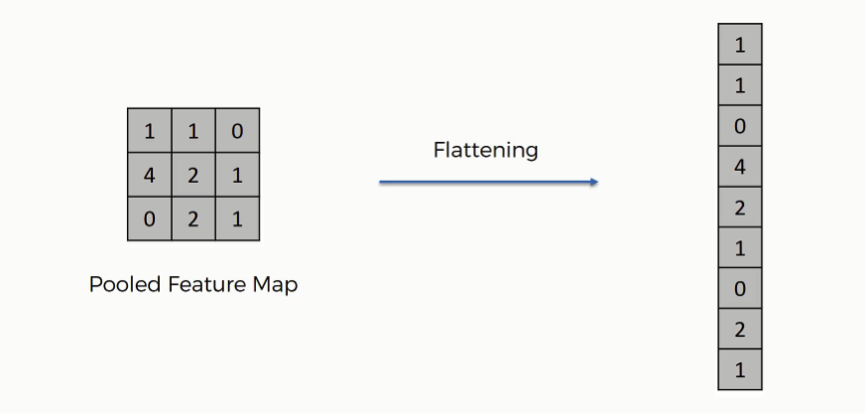
\includegraphics[scale=0.8]{images/flatten.png}
  \caption{Flattening}
  \label{fig:flatten}
\end{figure}